
\documentclass[12pt]{article}


\usepackage[T1]{fontenc}
\usepackage{amsfonts, amsmath, amssymb}
\usepackage{authblk}
\usepackage{multirow}
\usepackage{epsfig}
\usepackage{subfigure}
\usepackage{subfloat}
\usepackage{graphicx}
\usepackage{lscape}
\usepackage{amsmath}

\usepackage{amssymb}
\usepackage{gensymb}
\usepackage{tabularx}

\usepackage{booktabs}
\usepackage{longtable}
\usepackage{verbatim, rotating, paralist}
\usepackage{enumerate}
\usepackage{natbib}
\usepackage{multibib}
\usepackage{pdfsync}
\usepackage{latexsym}
\usepackage{amsthm}


\usepackage{stmaryrd}
\usepackage{dsfont}
\usepackage{hyperref}
\usepackage{bbm}
\usepackage{mathtools}

\usepackage{parskip}
\usepackage{anysize, indentfirst, setspace}
\usepackage[right=2.1cm, left=2.1cm, top=2.25cm, bottom=2.25cm]{geometry}
\usepackage{tikz}
\usepackage{epigraph}
\usepackage{csquotes}
\usepackage{appendix}
\usepackage{enumitem}
\usepackage{rotating}
\usepackage{changepage}


\renewcommand{\topfraction}{.85}
\renewcommand{\bottomfraction}{.7}
\renewcommand{\textfraction}{.15}
\renewcommand{\floatpagefraction}{.66}
\renewcommand{\dbltopfraction}{.66}
\renewcommand{\dblfloatpagefraction}{.66}

\usetikzlibrary{arrows,shapes,backgrounds,positioning,patterns,decorations.pathreplacing}
\newenvironment{shift}{\begin{adjustwidth}{1cm}{}}{\end{adjustwidth}}
\setlist{nosep}
\newcites{sec}{Appendix References}

%\renewcommand{\footnotelayout}{\doublespacing}
%\linespread{1.5}

%-----------------------------------BEGIN DOCUMENT--------------------------------%
\begin{document}

%----------------------------------------------------------------------------%
%---------------------------------APPENDIX-----------------------------------%
%----------------------------------------------------------------------------%

\normalsize

\appendix

%TC:ignore
%\begin{refsection}
%\nocitesec{*}



\clearpage

\begin{center}
\singlespacing
	\section*{\normalfont \LARGE Online Appendix to \\``Enfranchisement and Incarceration \\ After the 1965 Voting Rights Act''}

	\normalsize
	\vspace{.2in}
	{Appendix is for online publication only.}


	\large
	\vspace{.25in}
	Date: October 8th, 2021

\end{center}


\vspace{.2in}
\singlespacing
\normalsize

\setcounter{footnote}{0}
\setcounter{equation}{0}

\renewcommand{\thesubsection}{\Alph{subsection}}

\singlespacing
\noindent \textbf{Appendix Contents} \\


\noindent \textbf{A} \hspace*{.186in} \textbf{Brief History of Race, Franchise and Carceral State} \dotfill page~\pageref{appendix_history}\\
\noindent \textbf{B} \hspace*{.2in} \textbf{Section 5 Coverage} \dotfill page~\pageref{appendix_coverage}\\
\noindent \textbf{C} \hspace*{.2in} \textbf{Trends in Black Admission Rates by State} \dotfill page~\pageref{appendix_Black_rates_states}\\
\noindent \textbf{D} \hspace*{.197in} \textbf{Trends in Difference in Black-White Admission Rates by States}  \dotfill page~\pageref{appendix_diff_rates_states}\\
\noindent \textbf{E} \hspace*{.22in} \textbf{Incarceration Imputations}  \dotfill page~\pageref{appendix_imputations}\\
\noindent \textbf{F} \hspace*{.24in} \textbf{State Results Dropping One State at a Time}  \dotfill page~\pageref{appendix_jackknife}\\
\noindent \textbf{G} \hspace*{.2in} \textbf{County-Level Analyses}  \dotfill page~\pageref{appendix_county}\\
\noindent \textbf{H} \hspace*{.2in} \textbf{Black Elected Officials}  \dotfill page~\pageref{appendix_beo}\\
\noindent \textbf{I} \hspace*{.26in} \textbf{Attitudes to Crime and the Carceral State}  \dotfill page~\pageref{appendix_attitudes}\\
\noindent \textbf{J} \hspace*{.25in} \textbf{Fisher Randomization Tests}  \dotfill page~\pageref{appendix_fisher}\\
\noindent \textbf{K} \hspace*{.2in} \textbf{Feasible Generalized Least Squares}  \dotfill page~\pageref{appendix_fgls}\\
\noindent \textbf{L} \hspace*{.24in} \textbf{Event Study Analysis}  \dotfill page~\pageref{appendix_eventstudy}\\
\noindent \textbf{M} \hspace*{.188in} \textbf{County Heterogeneity for Black minus White}  \dotfill page~\pageref{appendix_countyheterogeneity_blackminuswhite}\\
\noindent \textbf{N} \hspace*{.215in} \textbf{Robustness to Maximally Influential Perturbations}  \dotfill page~\pageref{appendix_broderick}\\


\singlespacing





%----------------------------- APPENDIX A: Sources ---------------------------------%
\section{Brief History of Race, Franchise and Carceral State}\label{appendix_history}
\setcounter{table}{0}
\setcounter{figure}{0}
\renewcommand{\thetable}{A\arabic{table}}
\renewcommand{\thefigure}{A\arabic{figure}}
\normalsize

Race, enfranchisement and incarceration have been interwoven throughout the history of the US, particularly in the history of the South.  This paper focuses on enfranchisement in 1965.  However, taking a longer historical view of the process allows us to contextualize those mid-20th century events as a potentially \emph{strategic} or \emph{reactive} shift, born out a long history in which the carceral state was an explicit tool chosen by White political elites to enforce their political, social and economic dominance.

The US was founded with legal allowance for slavery that kept Blacks in a form of private incarceration throughout the South.\footnote{Carceral institutions like local police forces emerged in relation to slavery \citepsec{Reichel:1992wk}.}  It took a Civil War and a constitutional amendment (the 13th) to seemingly resolve the question of slavery.  The rapid emancipation in 1865 of more than four million former slaves in the South crippled the established economic order, and threatened the racial hierarchy that had become institutionalized to protect the White planter elite and to limit class conflict in the highly unequal southern society \citepsec{DuBois:1998vn}.  The racial animosity that supported that hierarchy was not simply swept away with the abolition of slavery \citepsec{Hendrickson:2003kh,Acharya:2016tn}.

With emancipation, former slaves gained political rights, and used those rights to vote, and obtain political office \citepsec{Logan:2017up}.  Despite this ``brief moment in the sun,'' White racial animosity and economic hardship sought other institutional modalities.  Wrote one observer of the Reconstruction era that followed the Civil War: ``There is a kind of $\ldots$ lingering hope among many in the South that slavery will be re-galvanized in some shape or other'' \citepsec[140]{DuBois:1998vn}. And Whites indeed shifted their strategy, exploiting the exception in the 13th amendment that allowed slavery ``\emph{as punishment for a crime}'' to use carceral institutions---Black Codes and convict-leasing---to confine and control supposedly free Blacks \citepsec{Blackmon:2009wo,Muhammad:2011wf,Mazumder:2019tp}.\footnote{``They tried by their laws to make a worse slavery than there was before'' \citepsec[140]{DuBois:1998vn}. Thus, race-based violence went beyond a private phenomenon---e.g. lynching---to which the state at best turned a blind eye \citepsec{WellsBarnett:2005uj}.  As noted by \citetsec[p. 57]{Mickey:2015vh}, Southern ``rulers supplemented restrictions on civil liberties by directing, endorsing, or acquiescing in the \emph{physical coercion} of their subjects$\ldots$ through imprisonment, expulsion, and destruction of property [as well as] torture, murder, and state execution.''}  As one Union soldier stationed in Meridian, Mississippi wrote of the former slaveholders, ``It is their hope, and intention, under the guise of vagrant laws, to restore all of slavery but its name.''

In addition to the rise in race-specific incarceration, a new set of policies---Jim Crow---arose to segregate society and enforce a racial \emph{political} hierarchy that evaporated Reconstruction era Black political gains \citepsec{Foner:2003tz,Keele:2019wu}. In turn, the age of Black codes and convict-leasing evolved into a 20th century in which Black communities lacked access to political power, and as a consequence, unbiased law enforcement institutions.\footnote{``The absence of a significant Negro electorate$\ldots$ the result of a purposeful and effective effort on the part of State and local officials to deny the franchise to Negroes,'' wrote the 1965 US Civil Rights Commission report on Law Enforcement, ``ensures that sheriffs will be responsible only to the White community.''\citep[87]{USCCRUnitedStatesCommissiononCivilRights:1965wk}.  Blacks were absent from positions within law enforcement as well.}  Carceral institutions continued to be used differentially against Blacks as an implicitly state-sanctioned tool of social control---enforcing the political and social hierarchy that was Jim Crow \citepsec{Muhammad:2011wf}.\footnote{See also various US Commission on Civil Rights Reports \citepsec{UnitedStatesCommissiononCivilRights:1963vq,USCCRUnitedStatesCommissiononCivilRights:1965wk,USCCRUnitedStatesCommissiononCivilRights:1974vd,USCCRUnitedStatesCommissiononCivilRights:1976vg,UnitedStates:1982ty}.}

As the Civil Rights movement of the 1950s and 60s gained force, law enforcement turned against Blacks exercising their constitutional rights to assemble and protest.  It was on the heels of Bloody Sunday in Selma, Alabama in August 1965, that the VRA was signed into law.  In many ways, the law formally changed little, merely affirming existing Civil Rights law and Constitutional amendments.\footnote{For example, Section 2 prohibits the use of race-based devices to restrict the right to vote, a prohibition already on the books in the 15th Amendment.}  In practice, however, it signaled a new-found willingness of the federal government to enforce existing law, and provided new tools for it to so.  Section 5 of the VRA, in particular, allowed the federal government to require specific ``covered'' jurisdictions to submit any changes to their voting rules or practices for approval prior to them going into effect.\footnote{The initial jurisdictions experiencing coverage were Alabama, Alaska, Georgia, Louisiana, Mississippi, South Carolina, Virginia, and 39 of the counties in North Carolina.  Coverage was triggered by a formula set out in Section 4 of the Act.  See Appendix~\ref{appendix_coverage}.}  This effectively curbed a cat-and-mouse game that had pitted fast-moving southern innovations in voting discrimination against the lethargy and apathy of national political and judicial processes. Images of this violent repression were critical in coalescing national support for political change.

The consequence of the VRA was an enfranchisement of southern Blacks that eclipsed that of the Reconstruction Era \citepsec{CivilRightsCommission:1975vd,Fresh:2018td}.  But despite these gains, there were widespread structural barriers that still severely limited Black political efficacy \citepsec{CivilRightsCommission:1975vd,Jeffries:2009wq}.  And there were powerful undercurrents that actively resisted the racially progressive tide \citepsec{Ward:fI0BEV0u,McDonald:2003tz,Moye:2006we}.  One of the critical places that this resistance emerged was in law enforcement.  While peaceful civil disobedience in the Civil Rights movement successfully secured Blacks voting rights, it also provided a focal point around which to organize a new set of law and order policies that only thinly veiled their racially repressive motivations \citepsec{Weaver:2007vr}.  Protesters were cast as criminals, and new rhetoric, new laws, and new funding highlighted the maintenance of order as an issue of critical national importance even \emph{before} crime rates rose \citepsec{Thompson:2019wo}.

From the 1960s onwards, incarceration rates in the US rose astronomically (Figure~\ref{figure_national_trends}).  The consequences of this mass incarceration---particularly for communities of color---are substantial and well-documented.  Felon disenfranchisement has formally limited the political power of the formerly-incarcerated \citepsec{Manza:2008vp,Uggen:2016ul}; contact with criminal justice institutions, more generally, has been found to depress political engagement \citepsec{Weaver:2010vs}; felony convictions limit individuals' access to jobs and important government services \citepsec{Alexander:2012tj,Agan:2018uh}; cycles of crime, poverty, low educational attainment and poor health keep incarcerated communities down \citepsec{Burch:2014ug}; and the allocation of incarcerated populations further draws services away from the neediest communities \citepsec{BrownDean:2016wl}.

The temporal link between Black enfranchisement and incarceration trends has not gone unrecognized by scholars \citepsec{Weaver:2007vr,Alexander:2012tj,Murakawa:2014vj,Hinton:2016tb}.\footnote{Writes \citesec[235]{Thompson:2019wo}: ``...what is unique about high rates of incarceration today is neither the origins nor the demographic profile of those imprisoned.  What is noteworthy is merely its magnitude which, itself, is the result of \emph{a most deeply racialized response to the myriad freedom struggles of the 1960s.}''  Italics added.}   Political scholarship has tended to focus on \emph{national} explanations for the rise of the carceral state, and by virtue, trends in \emph{federal} incarceration.\footnote{Federal drug crimes, for example, have received a lot of attention.  But incarceration as a result of federal drug convictions make up only 9.7\% of all federal crimes, and federal crimes make up only 9.8\% of overall incarceration \citepsec{Sawyer:2020vl}(year 2020 figures).  While the current literature is \emph{not} monolithically nationalist in its focus, it has been the \emph{general} focus \citepsec{Weaver:2017uq}.  }  Yet, Figure~\ref{figure_national_trends} shows that it was the \emph{states} (and to a slightly lesser extent, localities) that were the primary contributors to mass incarceration.\footnote{There are three main criminal jurisdictions in the US in which the carceral state operates.  The first is federal.  Federal law, federal police (the FBI), federal courts, and federal prisons comprise this domain.  The second is state.  State law, state and local police, state courts, and state prisons comprise this domain.  The final domain is local.  County ordinances and municipal codes, county and municipal police, county and municipal courts, and local jails comprise this final domain.  It's worth noting that these domains are not perfectly separate. State police, county police, and city police all enforce state law, for instance.  State crimes may be referred to the federal level for additional charges, as another example of overlap.}  Our paper focuses on this lesser studied, but dominant trend in state-level incarceration, and its place within a longer history of Black struggles for enfranchisement and repression by Whites.  ``Racial violence against Negroes in the South is lawlessness with a history and a purpose,'' wrote the 1965 US Civil Rights Commission Report on Law Enforcement.  ``First, with explicit and then with implicit legal sanction, violence has been used since the early days of slavery to maintain and reinforce the traditional subservient position of the Negro.''\footnote{\citesec{USCCRUnitedStatesCommissiononCivilRights:1965wk}.}


%----------------------------- APPENDIX C: Coverage ---------------------------------%
\section{Section 5 Coverage}\label{appendix_coverage}
\setcounter{table}{0}
\setcounter{figure}{0}
\renewcommand{\thetable}{B\arabic{table}}
\renewcommand{\thefigure}{B\arabic{figure}}
\normalsize

There were multiple Voting Rights Acts in the US that resulted in different political jurisdictions experiencing coverage---that is being subjected to the preclearance requirement originally contained in Section 5 of the 1965 version of the Act.  The formula used in determining coverage is described in Section 4 of the 1965 VRA.  If the jurisdiction maintained a ``test or device'' that was required in order to register to vote, it was covered.  These tests and devices included literacy tests, grandfather clauses, and poll taxes, among others.  In addition, if less than 50\% of the voting age population was registered to vote in November 1964, \emph{or} if less than 50\% of the voting age population turned out to vote, then the jurisdiction was covered.\footnote{Note that these were not race-specific triggers.}

Table~\ref{table_coverage} describes the jurisdictions covered by the 1965 VRA and two subsequent iterations of the Act.  The VRA was renewed on numerous occasions.  In 2013 the \emph{Shelby v Holder} Supreme Court decision struck down the continued application of Section 5 coverage based on the original Section 4 criteria effectively eliminating the practice of preclearance.


% Coverage Table
%-----------------
\begin{table}[h!] \scriptsize
\def\sym#1{\ifmmode^{#1}\else\(^{#1}\)\fi}
	\caption{Coverage}\label{table_coverage}
	\smallskip \centering
	\begin{tabular}{@{\extracolsep{5pt}} l l l}
	\noalign{\smallskip}\hline\hline\noalign{\smallskip}\noalign{\smallskip}
			\multicolumn{1}{c}{VRA} &  \multicolumn{1}{c}{States}  &  \multicolumn{1}{c}{Sub-State Jurisdictions} \\
			\midrule  \noalign{\smallskip}
      1965 & Alabama, Alaska, Georgia, & North Carolina  \\
          & Louisiana, Mississippi, South Carolina    & (39 counties) \\
          & Virginia \\
      \noalign{\smallskip}
      \noalign{\smallskip}
      1970 &  & California (2 counties), \\
           &  &  New York (3 counties), \\
           &  &  New Hampshire (10 townships) \\
      \noalign{\smallskip}
      \noalign{\smallskip}
      1975 &  Alaska, Arizona, Texas  &  California (3 counties), Florida (5 counties),   \\
           &   &   Michigan (2 townships), New York (2 counties), \\
           &   &  North Carolina (1 county),  \\
           &   & South Dakota (2 counties) \\
	     \hline\hline\noalign{\smallskip}
\multicolumn{3}{p{5.0in}}{\scriptsize  \emph{Notes}: Counties in Arizona, Hawaii and Idaho were initially designated for coverage in 1965, but almost immediately bailed out of coverage \citepsec[273]{Anonymous:1969tc}.  Counties in Connecticut, Idaho, Maine, Massachusetts and Wyoming were covered by the 1970 version of the act, but again, almost immediately bailed out of coverage \citepsec{USDepartmentofJustice:2020vh}.  The table does not include information on jurisdictions that were bailed out of coverage after having operated under coverage for a number of years.}
\end{tabular}
\end{table}







%--------------------- APPENDIX D: Black Rate State Plots -------------------------%
\vspace*{.2in}
\section{Trends in Black Admission Rates by State}\label{appendix_Black_rates_states}
\setcounter{table}{0}
\setcounter{figure}{0}
\renewcommand{\thetable}{C\arabic{table}}
\renewcommand{\thefigure}{C\arabic{figure}}
\normalsize

Figure~\ref{figure_states1} presents trends in Black prison admissions by state.  Points are raw data, trend lines are local polynomial fits. States in the South covered by Section 5 of the 1965-VRA have their trends presented in dashed grey.


% % %  FIGURE: State Black 1
% % %-------------------------------------------
\begin{figure}[h!]
 	\begin{center}
 	\caption{Trends in Black prison admissions rates by state}
 	\small

 		\vspace{.1in}
      \includegraphics[ width=2.0in, clip=true, trim=0.1in 0in 0.6in 0in ]{../../50_results/plot_AL.pdf}
 			\includegraphics[ width=2.0in, clip=true, trim=0.1in 0in 0.6in 0in  ]{../../50_results/plot_AZ.pdf}
       \includegraphics[ width=2.0in, clip=true, trim=0.1in 0in 0.6in 0in ]{../../50_results/plot_DE.pdf}\\

       \vspace{.01in}

 			\includegraphics[ width=2.0in, clip=true, trim=0.1in 0in 0.6in 0in  ]{../../50_results/plot_FL.pdf}
       \includegraphics[ width=2.0in, clip=true, trim=0.1in 0in 0.6in 0in  ]{../../50_results/plot_GA.pdf}
       \includegraphics[ width=2.0in, clip=true, trim=0.1in 0in 0.6in 0in ]{../../50_results/plot_KY.pdf}\\

       \vspace{.01in}

 			\includegraphics[ width=2.0in, clip=true, trim=0.1in 0in 0.6in 0in  ]{../../50_results/plot_LA.pdf}
 			\includegraphics[ width=2.0in, clip=true, trim=0.1in 0in 0.6in 0in ]{../../50_results/plot_MD.pdf}
 			\includegraphics[ width=2.0in, clip=true, trim=0.1in 0in 0.6in 0in  ]{../../50_results/plot_MO.pdf} \\

       \vspace{.01in}
       \includegraphics[ width=2.0in, clip=true, trim=0.1in 0in 0.6in 0in ]{../../50_results/plot_MS.pdf}
       \includegraphics[ width=2.0in, clip=true, trim=0.1in 0in 0.6in 0in  ]{../../50_results/plot_NC.pdf}
       \includegraphics[ width=2.0in, clip=true, trim=0.1in 0in 0.6in 0in  ]{../../50_results/plot_NM.pdf} \\

       \vspace{.01in}
       \includegraphics[ width=2.0in, clip=true, trim=0.1in 0in 0.6in 0in ]{../../50_results/plot_OK.pdf}
 			\includegraphics[ width=2.0in, clip=true, trim=0.0in 0in 0.7in 0in  ]{../../50_results/plot_SC.pdf}
 			\includegraphics[ width=2.0in, clip=true, trim=0.1in 0in 0.6in 0in  ]{../../50_results/plot_TN.pdf}\\

			\vspace{.01in}
			\includegraphics[ width=2.0in, clip=true, trim=0.1in 0in 0.6in 0in ]{../../50_results/plot_TX.pdf}
 			\includegraphics[ width=2.0in, clip=true, trim=0.1in 0in 0.6in 0in  ]{../../50_results/plot_VA.pdf}
       \includegraphics[ width=2.0in, clip=true, trim=0.1in 0in 0.6in 0in  ]{../../50_results/plot_WV.pdf}
			 \smallskip
 	\label{figure_states1}
 	\end{center}
   {\scriptsize{\emph{Notes:} Plots present the number of new Black prison admits as a percentage of the statewide Black population and local polynomial regression fits.  States in the South covered by Section 5 of the 1965-VRA have their trends presented in dashed grey. The y-axis scales are different for each plot.}}
 \end{figure} \normalsize

\clearpage













% %--------------------------- APPENDIX E: Difference B-W --------------------------------%
 \section{Trends in Difference in Black-White Admission Rates by States}\label{appendix_diff_rates_states}
 \setcounter{table}{0}
 \setcounter{figure}{0}
 \renewcommand{\thetable}{D\arabic{table}}
 \renewcommand{\thefigure}{D\arabic{figure}}
 \normalsize

Figure~\ref{figure_difference_states1} presents trends in the difference in Black-White prison admissions by state.  Black lines are the difference.  Black prison admissions are in dashed gray lines; White prison admissions are the dotted gray line.

 %  FIGURE: Difference 1
 %-------------------------
 \begin{figure}[h!]
 	\begin{center}
 	\caption{Trends in difference between Black and White prison admissions rates by state}
 	\small

 		\vspace{.1in}
       \includegraphics[ width=2.0in, clip=true, trim=0.1in 0in 0.6in 0in ]{../../50_results/plot_state_diff_AL.pdf}
 		\includegraphics[ width=2.0in, clip=true, trim=0.1in 0in 0.6in 0in  ]{../../50_results/plot_state_diff_AZ.pdf}
       \includegraphics[ width=2.0in, clip=true, trim=0.1in 0in 0.6in 0in ]{../../50_results/plot_state_diff_DE.pdf}\\

       \vspace{.01in}
 			\includegraphics[ width=2.0in, clip=true, trim=0.1in 0in 0.6in 0in  ]{../../50_results/plot_state_diff_FL.pdf}
       \includegraphics[ width=2.0in, clip=true, trim=0.1in 0in 0.6in 0in  ]{../../50_results/plot_state_diff_GA.pdf}
       \includegraphics[ width=2.0in, clip=true, trim=0.1in 0in 0.6in 0in ]{../../50_results/plot_state_diff_KY.pdf}\\

       \vspace{.01in}
      \includegraphics[ width=2.0in, clip=true, trim=0.1in 0in 0.6in 0in  ]{../../50_results/plot_state_diff_LA.pdf}
 			\includegraphics[ width=2.0in, clip=true, trim=0.1in 0in 0.6in 0in ]{../../50_results/plot_state_diff_MD.pdf}
 			\includegraphics[ width=2.0in, clip=true, trim=0.1in 0in 0.6in 0in  ]{../../50_results/plot_state_diff_MO.pdf} \\

       \vspace{.01in}
       \includegraphics[ width=2.0in, clip=true, trim=0.1in 0in 0.6in 0in ]{../../50_results/plot_state_diff_MS.pdf}
       \includegraphics[ width=2.0in, clip=true, trim=0.1in 0in 0.6in 0in  ]{../../50_results/plot_state_diff_NC.pdf}
       \includegraphics[ width=2.0in, clip=true, trim=0.1in 0in 0.6in 0in  ]{../../50_results/plot_state_diff_NM.pdf}\\

       \vspace{.01in}
       \includegraphics[ width=2.0in, clip=true, trim=0.1in 0in 0.6in 0in ]{../../50_results/plot_state_diff_OK.pdf}
 			\includegraphics[ width=2.0in, clip=true, trim=0.0in 0in 0.7in 0in  ]{../../50_results/plot_state_diff_SC.pdf}
 			\includegraphics[ width=2.0in, clip=true, trim=0.1in 0in 0.6in 0in  ]{../../50_results/plot_state_diff_TN.pdf}
       \smallskip
 	\label{figure_difference_states1}
 	\end{center}
   {\singlespacing \scriptsize{\emph{Notes:} Plots present local polynomial fits for difference between the rate of new Black prison admissions and new White prison admissions (Black line).  The rate of new Black prison admission is presented in dashed gray, while the rate of new White prison admissions is presented in dotted gray. Note that the y-axis scales are different for each plot.}}
\end{figure} \normalsize






 \newpage
 %  FIGURE: Difference 2
 %-------------------------------------------
 \begin{figure}[h!]
 	\begin{center}
 	\caption{Trends in difference between Black and White prison admissions rates by state (continued)}
 	\small

 		\vspace{.1in}
 			\includegraphics[ width=2.0in, clip=true, trim=0.1in 0in 0.6in 0in ]{../../50_results/plot_state_diff_TX.pdf}
 			\includegraphics[ width=2.0in, clip=true, trim=0.1in 0in 0.6in 0in  ]{../../50_results/plot_state_diff_VA.pdf}
       \includegraphics[ width=2.0in, clip=true, trim=0.1in 0in 0.6in 0in  ]{../../50_results/plot_state_diff_WV.pdf} \\
       \smallskip\smallskip\smallskip
 	\label{figure_difference_states2}
 	\end{center}
   {\scriptsize{\emph{Notes:} Plots present the difference between the rate of new Black prison admissions and new White prison admissions (Black line).  The rate of new Black prison admission is presented in dashed gray, while the rate of new White prison admissions is presented in dotted gray.  Note that the y-axis scales are different for each plot.}}
 \end{figure} \normalsize




 %----------------- APPENDIX F: INTERPOLATIONS ------------------------------------%
 \section{Incarceration Imputations}\label{appendix_imputations}
 \setcounter{table}{0}
 \setcounter{figure}{0}
 \renewcommand{\thetable}{E\arabic{table}}
 \renewcommand{\thefigure}{E\arabic{figure}}
 \normalsize

Imputation of missing incarceration data at the state level is accomplished through a multi-step process. Following \citesec{Honaker:2010wb}, we first estimate a local polynomial regression for each state to model the relationship between incarceration rates and time. Second, those predicted values are then fed into \emph{Amelia II} \citepsec{Honaker:2011ct} along with state and year fixed effects to model the missing incarceration data. Finally, \emph{Amelia II} generates a set of 20 datasets for our state-level estimates (10 for counties), each with missing values filled using values drawn from the modeled posterior distribution of missing values. Regressions are then run on each of these five datasets, and the parameters estimated from those regressions are then recombined to account for variation in parameter estimates caused by the estimation uncertainty of missing data imputations. Tables~\ref{figure_interpolation_0} and~\ref{figure_interpolation_1} show the source of each observation from the balanced panel dataset used for estimation of Table~\ref{table_state}.

% Note that the footnotes for these are in the stata code
% in 17_restricted_st_sample_summarystats.do
% labels are: figure_interpolation_0 and figure_interpolation_1.
\begin{table}[hb] \centering
\newcolumntype{C}{>{\centering\arraybackslash}X}

\caption{Prison Admission Observation Sources, Uncovered States}
\label{figure_interpolation_0}
{\scriptsize
\begin{tabularx}{\textwidth}{lCCCCCCCCCCC}

\toprule
{Year}&{AZ}&{DE}&{FL}&{KY}&{MD}&{MO}&{NM}&{OK}&{TN}&{TX}&{WV} \tabularnewline
\midrule\addlinespace[1.5ex]
1946&IC&IC&IC&IC&IC&IC&IC&IC&IC&IC&IC \tabularnewline
1947&$\cdot$&$\cdot$&$\cdot$&$\cdot$&$\cdot$&$\cdot$&$\cdot$&$\cdot$&$\cdot$&$\cdot$&$\cdot$ \tabularnewline
1948&$\cdot$&$\cdot$&$\cdot$&$\cdot$&$\cdot$&$\cdot$&$\cdot$&$\cdot$&$\cdot$&$\cdot$&$\cdot$ \tabularnewline
1949&$\cdot$&$\cdot$&AC&$\cdot$&$\cdot$&$\cdot$&$\cdot$&$\cdot$&$\cdot$&$\cdot$&$\cdot$ \tabularnewline
1950&IC&IC&IC&IC&IC&IC&IC&IC&IC&IC&IC \tabularnewline
1951&$\cdot$&$\cdot$&AC&$\cdot$&$\cdot$&$\cdot$&$\cdot$&$\cdot$&$\cdot$&$\cdot$&$\cdot$ \tabularnewline
1952&$\cdot$&$\cdot$&$\cdot$&$\cdot$&$\cdot$&$\cdot$&$\cdot$&$\cdot$&$\cdot$&$\cdot$&$\cdot$ \tabularnewline
1953&$\cdot$&$\cdot$&AC&$\cdot$&$\cdot$&$\cdot$&$\cdot$&$\cdot$&$\cdot$&$\cdot$&$\cdot$ \tabularnewline
1954&$\cdot$&$\cdot$&$\cdot$&$\cdot$&$\cdot$&$\cdot$&$\cdot$&$\cdot$&$\cdot$&$\cdot$&$\cdot$ \tabularnewline
1955&$\cdot$&$\cdot$&AC&$\cdot$&$\cdot$&$\cdot$&$\cdot$&$\cdot$&$\cdot$&$\cdot$&$\cdot$ \tabularnewline
1956&$\cdot$&$\cdot$&$\cdot$&$\cdot$&$\cdot$&$\cdot$&$\cdot$&$\cdot$&$\cdot$&$\cdot$&$\cdot$ \tabularnewline
1957&$\cdot$&$\cdot$&AC&$\cdot$&$\cdot$&$\cdot$&$\cdot$&$\cdot$&$\cdot$&$\cdot$&$\cdot$ \tabularnewline
1958&$\cdot$&$\cdot$&AC&$\cdot$&$\cdot$&$\cdot$&$\cdot$&$\cdot$&$\cdot$&$\cdot$&$\cdot$ \tabularnewline
1959&$\cdot$&$\cdot$&$\cdot$&$\cdot$&$\cdot$&$\cdot$&$\cdot$&$\cdot$&$\cdot$&$\cdot$&$\cdot$ \tabularnewline
1960&IC&IC&IC&IC&IC&IC&IC&IC&IC&IC&IC \tabularnewline
1961&$\cdot$&$\cdot$&AC&$\cdot$&$\cdot$&$\cdot$&$\cdot$&$\cdot$&$\cdot$&$\cdot$&$\cdot$ \tabularnewline
1962&$\cdot$&$\cdot$&AC&$\cdot$&$\cdot$&$\cdot$&$\cdot$&$\cdot$&AC&$\cdot$&$\cdot$ \tabularnewline
1963&$\cdot$&$\cdot$&AC&$\cdot$&$\cdot$&$\cdot$&$\cdot$&$\cdot$&$\cdot$&$\cdot$&$\cdot$ \tabularnewline
1964&IC&IC&IC&IC&IC&IC&IC&IC&IC&IC&IC \tabularnewline
1965&$\cdot$&$\cdot$&AC&$\cdot$&$\cdot$&$\cdot$&$\cdot$&$\cdot$&AC&$\cdot$&$\cdot$ \tabularnewline
1966&$\cdot$&$\cdot$&AC&$\cdot$&$\cdot$&$\cdot$&$\cdot$&$\cdot$&$\cdot$&$\cdot$&$\cdot$ \tabularnewline
1967&$\cdot$&$\cdot$&AC&$\cdot$&$\cdot$&$\cdot$&$\cdot$&$\cdot$&$\cdot$&$\cdot$&$\cdot$ \tabularnewline
1968&$\cdot$&$\cdot$&AC&$\cdot$&$\cdot$&$\cdot$&$\cdot$&$\cdot$&AC&$\cdot$&$\cdot$ \tabularnewline
1969&$\cdot$&$\cdot$&$\cdot$&$\cdot$&$\cdot$&$\cdot$&$\cdot$&$\cdot$&$\cdot$&$\cdot$&$\cdot$ \tabularnewline
1970&IC&IC&$\cdot$&IC&IC&IC&IC&IC&IC&$\cdot$&IC \tabularnewline
1971&$\cdot$&$\cdot$&$\cdot$&$\cdot$&$\cdot$&$\cdot$&$\cdot$&$\cdot$&$\cdot$&$\cdot$&$\cdot$ \tabularnewline
1972&$\cdot$&$\cdot$&$\cdot$&$\cdot$&$\cdot$&$\cdot$&$\cdot$&$\cdot$&$\cdot$&$\cdot$&$\cdot$ \tabularnewline
1973&$\cdot$&$\cdot$&$\cdot$&$\cdot$&$\cdot$&$\cdot$&$\cdot$&$\cdot$&$\cdot$&$\cdot$&$\cdot$ \tabularnewline
1974&IC&$\cdot$&AC&IC&$\cdot$&IC&IC&$\cdot$&IC&$\cdot$&$\cdot$ \tabularnewline
1975&IC&IC&AC&IC&$\cdot$&$\cdot$&IC&$\cdot$&IC&$\cdot$&$\cdot$ \tabularnewline
1976&IC&IC&AC&IC&$\cdot$&IC&IC&$\cdot$&IC&IC&IC \tabularnewline
1977&IC&IC&AC&IC&$\cdot$&IC&$\cdot$&$\cdot$&IC&IC&$\cdot$ \tabularnewline
1978&IC&IC&AC&IC&IC&IC&IC&$\cdot$&$\cdot$&IC&IC \tabularnewline
1979&$\cdot$&$\cdot$&$\cdot$&IC&$\cdot$&IC&IC&$\cdot$&$\cdot$&IC&IC \tabularnewline
1980&IC&IC&AC&IC&IC&IC&$\cdot$&$\cdot$&IC&IC&IC \tabularnewline
1981&$\cdot$&$\cdot$&AC&$\cdot$&$\cdot$&$\cdot$&$\cdot$&$\cdot$&AC&$\cdot$&$\cdot$ \tabularnewline
1982&$\cdot$&IC&AC&IC&$\cdot$&IC&IC&$\cdot$&IC&IC&IC \tabularnewline
\bottomrule \addlinespace[1.5ex]

\end{tabularx}
\begin{flushleft}
\scriptsize Table reports the source of prison admission values for each state-year. IC denotes observations that come from the ICPSR prison admissions dataset. AC denotes observations that were author collected from state archives. $\cdot$ denotes observations filled by multiple imputation. Note that some series appear to begin or end with interpolated values. In these cases, values were imputed using data from before or after the period for which we have a balanced panel -- prison admissions are not extrapolated.
\end{flushleft}
}
\end{table}

\begin{table}[hb] \centering
\newcolumntype{C}{>{\centering\arraybackslash}X}

\caption{Prison Admission Observation Sources, Covered States}
\label{figure_interpolation_1}
{\scriptsize
\begin{tabularx}{\textwidth}{lCCCCCCC}

\toprule
{Year}&{AL}&{GA}&{LA}&{MS}&{NC}&{SC}&{VA} \tabularnewline
\midrule\addlinespace[1.5ex]
1946&IC&IC&IC&$\cdot$&IC&IC&IC \tabularnewline
1947&$\cdot$&$\cdot$&AC&$\cdot$&$\cdot$&$\cdot$&$\cdot$ \tabularnewline
1948&$\cdot$&$\cdot$&AC&$\cdot$&$\cdot$&$\cdot$&$\cdot$ \tabularnewline
1949&$\cdot$&$\cdot$&AC&$\cdot$&$\cdot$&$\cdot$&AC \tabularnewline
1950&IC&AC&IC&IC&IC&IC&IC \tabularnewline
1951&$\cdot$&AC&AC&$\cdot$&AC&$\cdot$&AC \tabularnewline
1952&$\cdot$&$\cdot$&AC&$\cdot$&AC&$\cdot$&AC \tabularnewline
1953&$\cdot$&AC&$\cdot$&$\cdot$&AC&$\cdot$&AC \tabularnewline
1954&AC&AC&$\cdot$&$\cdot$&AC&$\cdot$&AC \tabularnewline
1955&$\cdot$&AC&$\cdot$&$\cdot$&AC&$\cdot$&AC \tabularnewline
1956&$\cdot$&$\cdot$&AC&$\cdot$&AC&$\cdot$&$\cdot$ \tabularnewline
1957&$\cdot$&$\cdot$&AC&$\cdot$&$\cdot$&$\cdot$&AC \tabularnewline
1958&$\cdot$&AC&AC&$\cdot$&$\cdot$&$\cdot$&$\cdot$ \tabularnewline
1959&$\cdot$&AC&AC&$\cdot$&AC&$\cdot$&$\cdot$ \tabularnewline
1960&IC&IC&IC&IC&IC&IC&IC \tabularnewline
1961&AC&$\cdot$&AC&$\cdot$&AC&$\cdot$&AC \tabularnewline
1962&AC&AC&AC&$\cdot$&AC&$\cdot$&$\cdot$ \tabularnewline
1963&AC&AC&AC&$\cdot$&AC&$\cdot$&AC \tabularnewline
1964&IC&IC&IC&IC&IC&IC&IC \tabularnewline
1965&AC&AC&AC&$\cdot$&$\cdot$&$\cdot$&AC \tabularnewline
1966&AC&AC&$\cdot$&$\cdot$&$\cdot$&$\cdot$&AC \tabularnewline
1967&AC&AC&$\cdot$&$\cdot$&$\cdot$&$\cdot$&AC \tabularnewline
1968&AC&AC&$\cdot$&$\cdot$&$\cdot$&$\cdot$&$\cdot$ \tabularnewline
1969&AC&AC&$\cdot$&$\cdot$&AC&$\cdot$&AC \tabularnewline
1970&AC&IC&$\cdot$&IC&AC&IC&AC \tabularnewline
1971&AC&AC&$\cdot$&$\cdot$&AC&$\cdot$&AC \tabularnewline
1972&AC&AC&$\cdot$&$\cdot$&AC&AC&AC \tabularnewline
1973&$\cdot$&AC&$\cdot$&$\cdot$&AC&AC&AC \tabularnewline
1974&IC&IC&IC&$\cdot$&AC&AC&AC \tabularnewline
1975&IC&AC&AC&IC&AC&$\cdot$&AC \tabularnewline
1976&IC&AC&AC&IC&AC&$\cdot$&AC \tabularnewline
1977&AC&IC&AC&$\cdot$&AC&$\cdot$&AC \tabularnewline
1978&AC&IC&AC&$\cdot$&IC&IC&AC \tabularnewline
1979&AC&IC&AC&IC&IC&IC&AC \tabularnewline
1980&IC&IC&AC&IC&IC&IC&AC \tabularnewline
1981&$\cdot$&AC&AC&$\cdot$&$\cdot$&AC&AC \tabularnewline
1982&IC&IC&AC&IC&IC&IC&AC \tabularnewline
\bottomrule \addlinespace[1.5ex]

\end{tabularx}
\begin{flushleft}
\scriptsize Table reports the source of prison admission values for each state-year. IC denotes observations that come from the ICPSR prison admissions dataset. AC denotes observations that were author collected from state archives. $\cdot$ denotes observations filled by multiple imputation. Note that some series appear to begin or end with interpolated values. In these cases, values were imputed using data from before or after the period for which we have a balanced panel -- prison admissions are not extrapolated.
\end{flushleft}
}
\end{table}


\clearpage


%--------------------------- APPENDIX F: Jackknife ----------------------------%
\section{State Results Dropping One State at a Time}\label{appendix_jackknife}
\setcounter{table}{0}
\setcounter{figure}{0}
\renewcommand{\thetable}{F\arabic{table}}
\renewcommand{\thefigure}{F\arabic{figure}}
\normalsize

In this appendix, we present results for the estimates of our main parameter of interest when we iteratively drop one state from our analysis sample.  This helps ensure that despite our small sample of states, our effect sizes and statistical significance are not the results of a single outlier state.

Figure~\ref{figure_jackknife_black} presents the point estimates and 90\% confidence intervals from our long-difference version of our two-way fixed effects model (Plot (a)), and the distribution of those estimates (Plot (b)) for our Black admissions rate outcome. Figure~\ref{figure_jackknife_bminusw} presents the same plots but for our difference between Black and White admissions rates outcome.  In both cases, we find our point estimates are substantively quite stable, and while the exclusion of some states does cause our statistical significance to fall below the 0.05 threshold, the magnitude of these shifts are relatively small, and some fall in significance is to be expected given we are dropping 1 of only 18 states in these specifications.

% %  Jackknife: Black
% %-------------------------------------------
\begin{figure}[h!]
 	\begin{center}
 	\caption{ Plots for iteratively dropping one state for estimates of Black admissions rate }
 	\footnotesize
		(a) Long Difference Point Estimates \hspace*{.4in} (b) Distribution of Point Estimates \\
 			\includegraphics[ width=3.13in, clip=true, trim=0.1in 0in 0.6in 0in ]{../../50_results/jackknife_bminusw_points_ols.pdf}
 			\includegraphics[ width=3.1in, clip=true, trim=0.1in 0in 0.6in 0in  ]{../../50_results/jackknife_bminusw_ols.pdf} \\
       \smallskip
       \label{figure_jackknife_black}
       \end{center}
\end{figure} \normalsize



% %  Jackknife: Black Minus White
% %-------------------------------------------
\begin{figure}[h!]
 	\begin{center}
 	\caption{ Plots for iteratively dropping one state for estimates of Black minus White admissions rate }
 	\footnotesize
		(a) Long Difference Point Estimates \hspace*{.4in} (b) Distribution of Point Estimates \\
 			\includegraphics[ width=3.1in, clip=true, trim=0.1in 0in 0.6in 0in ]{../../50_results/jackknife_black_points_ols.pdf}
 			\includegraphics[ width=3.1in, clip=true, trim=0.1in 0in 0.6in 0in  ]{../../50_results/jackknife_black_ols.pdf} \\
       \smallskip
       \label{figure_jackknife_bminusw}
       \end{center}
\end{figure} \normalsize







%------------------------ APPENDIX J: County something ------------------------%
\section{County Analyses}\label{appendix_county}
\setcounter{table}{0}
\setcounter{figure}{0}
\renewcommand{\thetable}{G\arabic{table}}
\renewcommand{\thefigure}{G\arabic{figure}}
\normalsize

As discussed in Section~\ref{section_blackpoliticalempowerment}, our analysis of county-level heterogeneity is limited by data availability. We were able to collect county-by-year-by-race data on state prison admissions for only six of the 18 states we study, and of these six, only the sample of Alabama, Georgia, and Tennessee exhibits similar overall dynamics to our full 18 state sample. This is demonstrated in Tables G1 and G2.\footnote{We explored all other sample permutations before settling on these three states as our most typical sample.} As our interest is in developing a deeper understanding of ``typical'' cases of the phenomenon we observe in our full sample, we therefore follow \citesec{Seawright:2008us} and focus on this sample of three states.

As shown in Tables G3 and G4, however, while there are differences in the estimate of average effects when we use all six states, we observe similar patterns of heterogeneity with both samples, providing some additional reassurance in our primary results.  The magnitudes of the estimates are the main difference.  Finally, Tables G5 and G6 presents the results of our analysis of county-level heterogeneity after splitting the sample by Black share of registered voters rather than share of population.


\begin{figure}[h!]
	\centering
	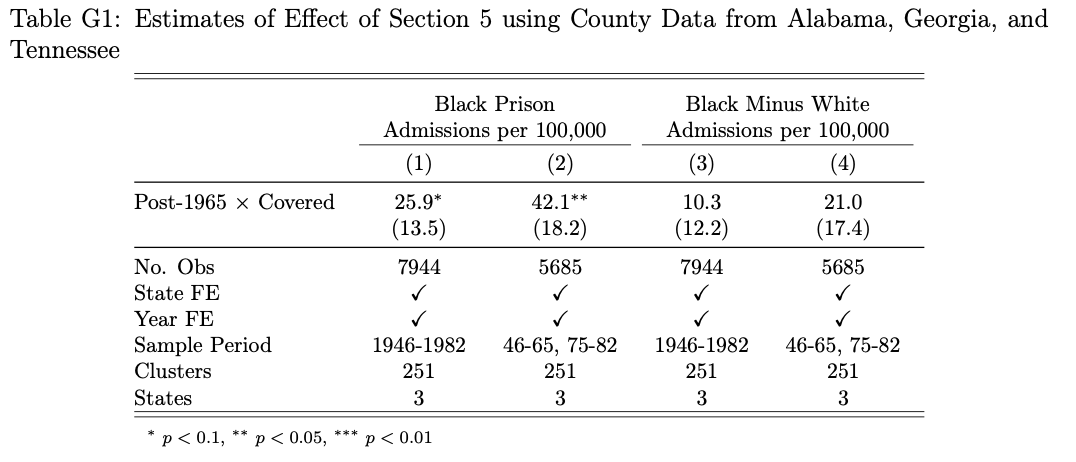
\includegraphics[width=6.3in]{../../60_appendix_cty_results/table_g1.png} \\
	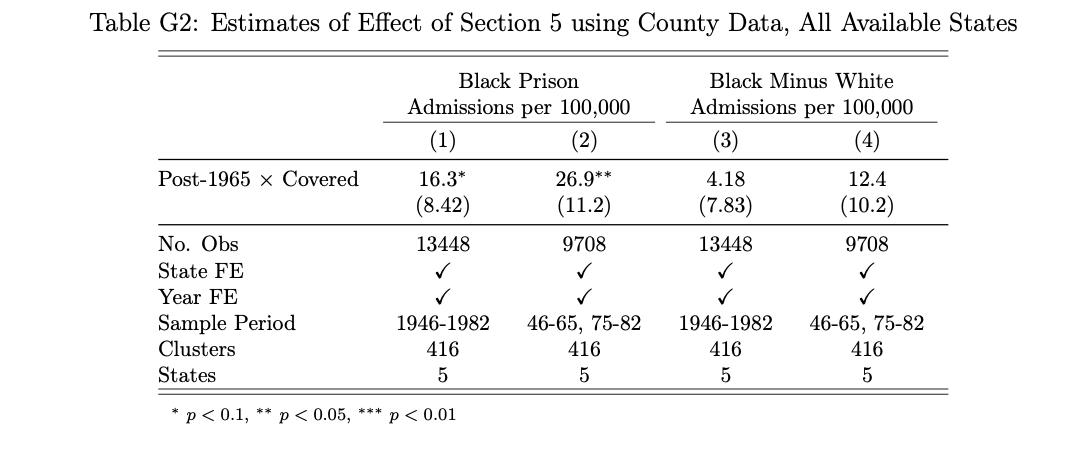
\includegraphics[width=6.3in]{../../60_appendix_cty_results/table_g2.png}
\end{figure}


\begin{figure}[h!]
	\centering
	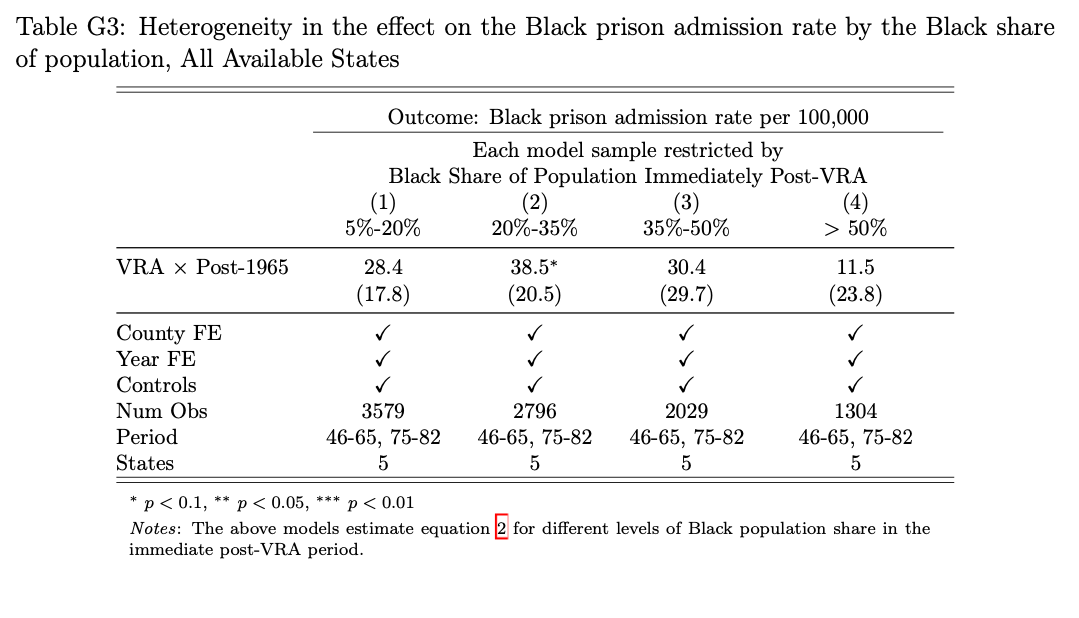
\includegraphics[width=5.9in, clip=true, trim=0.0in 0.8in 0in 0in]{../../60_appendix_cty_results/table_g3.png} \\
	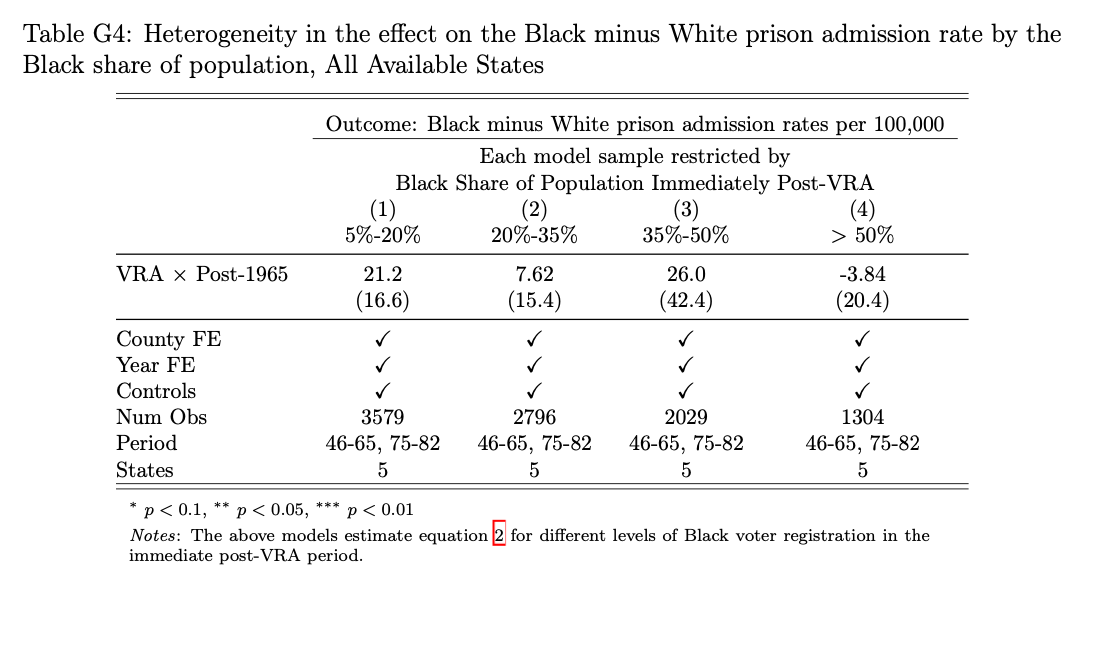
\includegraphics[width=5.9in, clip=true, trim=0.0in 0.8in 0in 0in]{../../60_appendix_cty_results/table_g4.png} \\
	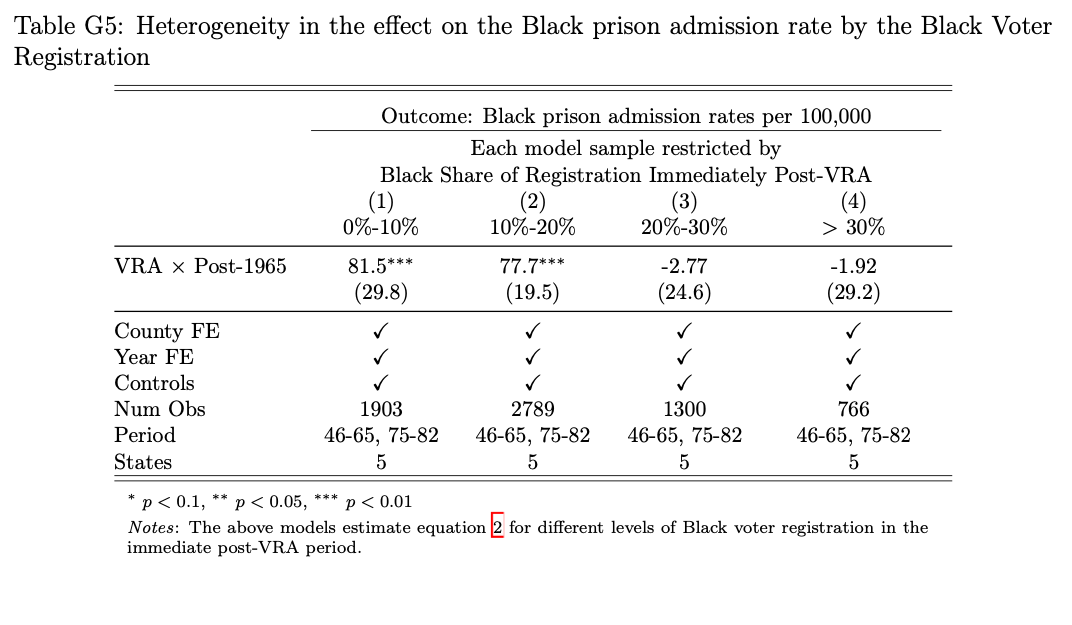
\includegraphics[width=5.9in]{../../60_appendix_cty_results/table_g5.png}
\end{figure}


\clearpage \newpage
\begin{figure}[h!]
	\centering
	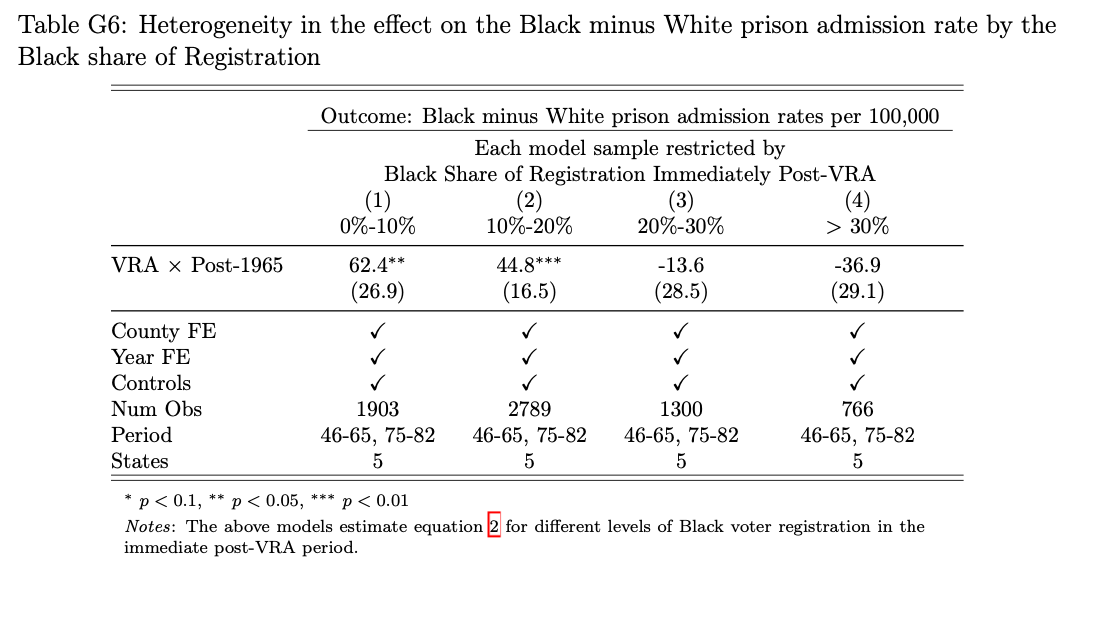
\includegraphics[width=6.0in]{../../60_appendix_cty_results/table_g6.png}
\end{figure}

% \begin{table}[h!]\centering \footnotesize
% \def\sym#1{\ifmmode^{#1}\else\(^{#1}\)\fi}
% 	\smallskip
% 	\begin{tabular}{@{\extracolsep{5pt}}l*{5}{c}}
% 	\noalign{\smallskip}\hline\hline\noalign{\smallskip}\noalign{\smallskip}
% 			&  \multicolumn{2}{c}{Black Prison }  & \multicolumn{2}{c}{Black Minus White}  \\
% 			&  \multicolumn{2}{c}{Admissions per 100,000} & \multicolumn{2}{c}{Admissions per 100,000}  \\
% 			\cline{2-3} \cline{4-5}   \noalign{\smallskip}
% 				                &\multicolumn{1}{c}{(1)}         &\multicolumn{1}{c}{(2)}         &\multicolumn{1}{c}{(3)}         &\multicolumn{1}{c}{(4)}         \\
\midrule
Post-1965 $\times$ Covered&     25.9\sym{*}  &     42.1\sym{**} &     10.3         &     21.0         \\
                &   (13.5)         &   (18.2)         &   (12.2)         &   (17.4)         \\
\midrule
No. Obs         &     7944         &     5685         &     7944         &     5685         \\
State FE        &\checkmark         &\checkmark         &\checkmark         &\checkmark         \\
Year FE         &\checkmark         &\checkmark         &\checkmark         &\checkmark         \\
Sample Period   &1946-82         &46-65, 75-82         &1946-82         &46-65, 75-82         \\
Clusters        &      251         &      251         &      251         &      251         \\
States          &        3         &        3         &        3         &        3         \\
 \\
% 	\noalign{\vspace*{-.17in}}\hline\hline\noalign{\smallskip}
% \multicolumn{5}{l}{\scriptsize \sym{*} \(p<0.1\), \sym{**} \(p<0.05\), \sym{***} \(p<0.01\)}\\
% \end{tabular}
% \end{table}


% \begin{table}[h!]\centering \footnotesize
% \def\sym#1{\ifmmode^{#1}\else\(^{#1}\)\fi}
% 	\caption{Estimates of Effect of Section 5 using County Data, All Available States}\label{table_county_allstates}
% 	\smallskip
% 	\begin{tabular}{@{\extracolsep{5pt}}l*{5}{c}}
% 	\noalign{\smallskip}\hline\hline\noalign{\smallskip}\noalign{\smallskip}
% 			&  \multicolumn{2}{c}{Black Prison }  & \multicolumn{2}{c}{Black Minus White}  \\
% 			&  \multicolumn{2}{c}{Admissions per 100,000} & \multicolumn{2}{c}{Admissions per 100,000}  \\
% 			\cline{2-3} \cline{4-5}   \noalign{\smallskip}
% 				                &\multicolumn{1}{c}{(1)}         &\multicolumn{1}{c}{(2)}         &\multicolumn{1}{c}{(3)}         &\multicolumn{1}{c}{(4)}         \\
\midrule
Post-1965 $\times$ Covered&     16.3\sym{*}         &    26.9\sym{**} &     4.18         &     12.4         \\
                &   (8.42)         &   (11.2)         &   (7.83)         &   (10.2)         \\
\midrule
No. Obs         &    13448         &     9708         &    13448         &     9708         \\
State FE        &\checkmark         &\checkmark         &\checkmark         &\checkmark         \\
Year FE         &\checkmark         &\checkmark         &\checkmark         &\checkmark         \\
Sample Period   &1946-82         &46-65, 75-82         &1946-82         &46-65, 75-82         \\
Clusters        &      416         &      416         &      416         &      416         \\
States          &        5         &        5         &        5         &        5         \\
 \\
% 	\noalign{\vspace*{-.17in}}\hline\hline\noalign{\smallskip}
% \multicolumn{5}{l}{\scriptsize \sym{*} \(p<0.1\), \sym{**} \(p<0.05\), \sym{***} \(p<0.01\)}\\
% \end{tabular}
% \end{table}

% % TABLE: Heterogeneity black voters Black admissions
% %---------------------------------------------------
% \begin{table}[h!]\centering \footnotesize
% \def\sym#1{\ifmmode^{#1}\else\(^{#1}\)\fi}
% 	\caption{Heterogeneity in the effect on the Black prison admission rate by the Black share of population, All Available States}\label{table_countyheterogeneity_allstates_black}
% 	\smallskip
% 	\begin{tabular}{@{\extracolsep{5pt}}l*{5}{c}}
% 			\noalign{\smallskip}\hline\hline\noalign{\smallskip}\noalign{\smallskip}
% 					&  \multicolumn{4}{c}{Outcome: Black prison admission rate per 100,000} \\
% 					\cline{2-5}   \noalign{\smallskip}
% 					&  \multicolumn{4}{c}{Each model sample restricted by} \\
% 					&  \multicolumn{4}{c}{Black Share of Population Immediately Post-VRA} \\
% 					                &\multicolumn{1}{c}{(1)}&\multicolumn{1}{c}{(2)}&\multicolumn{1}{c}{(3)}&\multicolumn{1}{c}{(4)}\\
                &\multicolumn{1}{c}{5\%-20\%}&\multicolumn{1}{c}{20\%-35\%}&\multicolumn{1}{c}{35\%-50\%}&\multicolumn{1}{c}{$>$ 50\%}\\
\midrule
VRA $\times$ Post-1965&     28.4         &     38.5\sym{*}  &     30.4         &     11.5        \\
                &   (17.8)         &   (20.5)         &   (29.7)         &   (23.8)         \\
\midrule
County FE       &\checkmark         &\checkmark         &\checkmark         &\checkmark         \\
Year FE         &\checkmark         &\checkmark         &\checkmark         &\checkmark         \\
Controls        &\checkmark         &\checkmark         &\checkmark         &\checkmark         \\
Num Obs         &     3579         &     2796         &     2029         &     1304         \\
Period          &46-65, 75-82         &46-65, 75-82         &46-65, 75-82         &46-65, 75-82         \\
States          &        5         &        5         &        5         &        5         \\
 \\
% 	\noalign{\vspace*{-.17in}}\hline\hline\noalign{\smallskip}
% 		\multicolumn{5}{l}{\scriptsize \sym{*} \(p<0.1\), \sym{**} \(p<0.05\), \sym{***} \(p<0.01\)}\\
% 		\multicolumn{5}{p{5.1in}}{\scriptsize  \emph{Notes}: The above models estimate equation~\ref{equation_dind_np} for different levels of Black population share in the immediate post-VRA period. }
% \end{tabular}
% \end{table}





% % TABLE: Heterogeneity black voters Black admissions
% %---------------------------------------------------
% \begin{table}[h!]\centering \footnotesize
% \def\sym#1{\ifmmode^{#1}\else\(^{#1}\)\fi}
% 	\caption{Heterogeneity in the effect on the Black minus White prison admission rate by the Black share of population, All Available States}\label{table_countyheterogeneity_allstates_bminusw}
% 	\smallskip
% 	\begin{tabular}{@{\extracolsep{5pt}}l*{5}{c}}
% 			\noalign{\smallskip}\hline\hline\noalign{\smallskip}\noalign{\smallskip}
% 					&  \multicolumn{4}{c}{Outcome: Black minus White prison admission rates per 100,000} \\
% 					\cline{2-5}   \noalign{\smallskip}
% 					&  \multicolumn{4}{c}{Each model sample restricted by} \\
% 					&  \multicolumn{4}{c}{Black Share of Population Immediately Post-VRA} \\
% 					                &\multicolumn{1}{c}{(1)}&\multicolumn{1}{c}{(2)}&\multicolumn{1}{c}{(3)}&\multicolumn{1}{c}{(4)}\\
                &\multicolumn{1}{c}{5\%-20\%}&\multicolumn{1}{c}{20\%-35\%}&\multicolumn{1}{c}{35\%-50\%}&\multicolumn{1}{c}{$>$ 50\%}\\
\midrule
VRA $\times$ Post-1965&     18.6         &     7.95         &     26.9         &    -2.50         \\
                &   (17.4)         &   (15.2)         &   (39.8)         &   (30.9)         \\
\midrule
County FE       &\checkmark         &\checkmark         &\checkmark         &\checkmark         \\
Year FE         &\checkmark         &\checkmark         &\checkmark         &\checkmark         \\
Controls        &\checkmark         &\checkmark         &\checkmark         &\checkmark         \\
Num Obs         &     3336         &     2662         &     1874         &     1229         \\
Period          &46-65, 75-82         &46-65, 75-82         &46-65, 75-82         &46-65, 75-82         \\
States          &        5         &        5         &        5         &        5         \\
 \\
% 	\noalign{\vspace*{-.17in}}\hline\hline\noalign{\smallskip}
% 		\multicolumn{5}{l}{\scriptsize \sym{*} \(p<0.1\), \sym{**} \(p<0.05\), \sym{***} \(p<0.01\)}\\
% 		\multicolumn{5}{p{5.1in}}{\scriptsize  \emph{Notes}: The above models estimate equation~\ref{equation_dind_np} for different levels of Black voter registration in the immediate post-VRA period. }
% \end{tabular}
% \end{table}


% % TABLE: Heterogeneity black voters Black admissions
% %---------------------------------------------------
% \begin{table}[h!]\centering \footnotesize
% \def\sym#1{\ifmmode^{#1}\else\(^{#1}\)\fi}
% 	\caption{Heterogeneity in the effect on the Black prison admission rate by the Black Voter Registration}\label{table_countyheterogeneity_reg_black}
% 	\smallskip
% 	\begin{tabular}{@{\extracolsep{5pt}}l*{5}{c}}
% 			\noalign{\smallskip}\hline\hline\noalign{\smallskip}\noalign{\smallskip}
% 					&  \multicolumn{4}{c}{Outcome: Black prison admission rates per 100,000} \\
% 					\cline{2-5}   \noalign{\smallskip}
% 					&  \multicolumn{4}{c}{Each model sample restricted by} \\
% 					&  \multicolumn{4}{c}{Black Share of Registration Immediately Post-VRA} \\
% 					                &\multicolumn{1}{c}{(1)}&\multicolumn{1}{c}{(2)}&\multicolumn{1}{c}{(3)}&\multicolumn{1}{c}{(4)}\\
                &\multicolumn{1}{c}{0\%-10\%}&\multicolumn{1}{c}{10\%-20\%}&\multicolumn{1}{c}{20\%-30\%}&\multicolumn{1}{c}{$>$ 30\%}\\
\midrule
VRA $\times$ Post-1965&     77.6\sym{**} &     74.4\sym{***}&    -3.13         &     1.46         \\
                &   (30.5)         &   (19.1)         &   (24.6)         &   (28.8)         \\
\midrule
County FE       &\checkmark         &\checkmark         &\checkmark         &\checkmark         \\
Year FE         &\checkmark         &\checkmark         &\checkmark         &\checkmark         \\
Controls        &\checkmark         &\checkmark         &\checkmark         &\checkmark         \\
Num Obs         &     1895         &     2777         &     1295         &      758         \\
Period          &46-65, 75-82         &46-65, 75-82         &46-65, 75-82         &46-65, 75-82         \\
States          &        5         &        5         &        5         &        5         \\
 \\
% 	\noalign{\vspace*{-.17in}}\hline\hline\noalign{\smallskip}
% 		\multicolumn{5}{l}{\scriptsize \sym{*} \(p<0.1\), \sym{**} \(p<0.05\), \sym{***} \(p<0.01\)}\\
% 		\multicolumn{5}{p{5.1in}}{\scriptsize  \emph{Notes}: The above models estimate equation~\ref{equation_dind_np} for different levels of Black voter registration in the immediate post-VRA period.  }
% \end{tabular}
% \end{table}



% \begin{table}[hb]\centering \footnotesize
% \def\sym#1{\ifmmode^{#1}\else\(^{#1}\)\fi}
% 	\caption{Heterogeneity in the effect on the Black minus White prison admission rate by the Black share of Registration}\label{table_countyheterogeneity_reg_bminusw}
% 	\smallskip
% 	\begin{tabular}{@{\extracolsep{5pt}}l*{5}{c}}
% 			\noalign{\smallskip}\hline\hline\noalign{\smallskip}\noalign{\smallskip}
% 					&  \multicolumn{4}{c}{Outcome: Black minus White prison admission rates per 100,000} \\
% 					\cline{2-5}   \noalign{\smallskip}
% 					&  \multicolumn{4}{c}{Each model sample restricted by} \\
% 					&  \multicolumn{4}{c}{Black Share of Registration Immediately Post-VRA} \\
% 					                &\multicolumn{1}{c}{(1)}&\multicolumn{1}{c}{(2)}&\multicolumn{1}{c}{(3)}&\multicolumn{1}{c}{(4)}\\
                &\multicolumn{1}{c}{0\%-10\%}&\multicolumn{1}{c}{10\%-20\%}&\multicolumn{1}{c}{20\%-30\%}&\multicolumn{1}{c}{$>$ 30\%}\\
\midrule
VRA $\times$ Post-1965&     55.9\sym{**} &     43.0\sym{***}&    -11.1         &    -27.3         \\
                &   (27.7)         &   (16.5)         &   (27.1)         &   (24.0)         \\
\midrule
County FE       &\checkmark         &\checkmark         &\checkmark         &\checkmark         \\
Year FE         &\checkmark         &\checkmark         &\checkmark         &\checkmark         \\
Controls        &\checkmark         &\checkmark         &\checkmark         &\checkmark         \\
Num Obs         &     1903         &     2789         &     1300         &      766         \\
Period          &46-65, 75-82         &46-65, 75-82         &46-65, 75-82         &46-65, 75-82         \\
States          &        5         &        5         &        5         &        5         \\
 \\
% 	\noalign{\vspace*{-.17in}}\hline\hline\noalign{\smallskip}
% 		\multicolumn{5}{l}{\scriptsize \sym{*} \(p<0.1\), \sym{**} \(p<0.05\), \sym{***} \(p<0.01\)}\\
% 		\multicolumn{5}{p{5.1in}}{\scriptsize  \emph{Notes}: The above models estimate equation~\ref{equation_dind_np} for different levels of Black voter registration in the immediate post-VRA period. }
% \end{tabular}
% \end{table}


%--------------------------- APPENDIX K: BEO --------------------------------%
\section{Black Elected Officials}\label{appendix_beo}
\setcounter{table}{0}
\setcounter{figure}{0}
\renewcommand{\thetable}{H\arabic{table}}
\renewcommand{\thefigure}{H\arabic{figure}}
\normalsize


Black political empowerment can take on a number of forms.  In the paper, we focus on conceptualizing and measuring empowerment in terms of electoral strength---the potential size of the Black electorate at the local level (measured by the Black percentage of the total population), and the observed strength of the Black electorate (measured by the share of total voter registrants who are Black).

Of course, the ability to obtain desired policy outcomes may be a function of more than just electoral strength.  Descriptive representation may substitute for such strength, augment it, or descriptive representation may even prove a \emph{necessary} condition for obtaining policy outcomes \citepsec{Preuhs:2006ww}.  Indeed much of the early work of organizations like the Student Non-Violent Coordinating Committee (SNCC) in the South was predicated \emph{not} on turning Blacks out to vote to induce accountability from White incumbents (or even new White candidates), but securing the election of Black candidates who Black voters could ``trust'' to have their interests at heart \citepsec{Jeffries:2009wq}.

Descriptive representation may matter generally across political offices, and it may play a particularly important role in positions most directly related to the carceral state \citepsec{Saltzstein:1989up}.  Local politicians may play a role in managing carceral budgets; organizing and overseeing carceral bureaucracies; and may even play a role in appointing key law enforcement officers.  Then, more specifically, when elected, Black sheriffs, prosecutors and judges can even more directly shape arrests, charges and sentences.

Thus, in addition to an interest in how our main results are conditioned by the electoral strength of Black communities, we are also interested in how those results are conditioned by the election of Black officials.  We want to know if the \emph{Self Policing} argument can explain the main results in our paper.  As with our other tests, for this to be the case, we are interested in whether, in those instances in which Blacks were \emph{most likely} to be able to translate their policy preferences into policy outcomes, we observe an increase in Black incarceration.  That is, does Black elected officeholding result in increased Black political incarceration.  Such evidence would suggest that enfranchisement allowed Black communities to obtain their desired carceral objectives.  Though, as with the size of the Black electorate, we note that Black officeholding is by no means a guarantee of Black policy efficacy;\footnote{For example, instances in which Black elected officials obtained a minority of elected positions may have appeared as a threat as much as evidence of Black political empowerment. } rather, we consider it the place Black communities are more \emph{likely} to be obtaining their preferences.


To examine this heterogeneity, we digitize and entered data from sixteen years of the \emph{Roster of Black Elected Officials} from 1969-1988 for the 11 states of the former Confederacy.\footnote{The 1977 volume was not published to our knowledge.  We also could not obtain the 1982, 1983, 1985 and 1986 volumes.  Resources limited our ability to collect data from a larger sample of states.}  Other scholars have also fruitfully worked with this data \citepsec{Bernini:2017tv,Aneja:2019uz}. These rosters contain entries for every Black official at the state and local level, including the position that they held, and where they held it.  Because the number of officials in the pre-1965 period is essential to being able to use a difference-in-differences design (as in the main paper), we use data presented in \citesec{Bernini:2017tv} on the count of pre-1965 Black elected officials.\footnote{We look at the map in their paper.}  We make the assumption that these are the only officials during the immediate pre-1965 period.  In our research, we have not come across evidence contrary to that assumption.






% %  FIGURE: BEO
% %-------------------------------------------
 \begin{figure}[h!]
 	\begin{center}
 	\caption{Trends in Black elected officials by type in the South}
 	\small
 		\vspace{.05in}
 			\includegraphics[ width=2.0in, clip=true, trim=0.1in 0in 0.05in 0in ]{../../50_results/plot_beo_AL.pdf}
 			\includegraphics[ width=2.0in, clip=true, trim=0.0in 0in 0.05in 0in  ]{../../50_results/plot_beo_AR.pdf}
 			\includegraphics[ width=2.0in, clip=true, trim=0.1in 0in 0.05in 0in  ]{../../50_results/plot_beo_FL.pdf}\\

       \vspace{.01in}
 			\includegraphics[ width=2.0in, clip=true, trim=0.1in 0in 0.05in 0in ]{../../50_results/plot_beo_GA.pdf}
 			\includegraphics[ width=2.0in, clip=true, trim=0.1in 0in 0.05in 0in  ]{../../50_results/plot_beo_LA.pdf}
      \includegraphics[ width=2.0in, clip=true, trim=0.1in 0in 0.05in 0in  ]{../../50_results/plot_beo_MS.pdf} \\

       \vspace{.01in}
 			\includegraphics[ width=2.0in, clip=true, trim=0.1in 0in 0.1in 0in ]{../../50_results/plot_beo_NC.pdf}
 			\includegraphics[ width=2.0in, clip=true, trim=0.1in 0in 0.05in 0in  ]{../../50_results/plot_beo_SC.pdf}
      \includegraphics[ width=2.0in, clip=true, trim=0.1in 0in 0.05in 0in  ]{../../50_results/plot_beo_TN.pdf} \\

      \vspace{.01in}
 			\includegraphics[ width=2.0in, clip=true, trim=0.1in 0in 0.05in 0in ]{../../50_results/plot_beo_TX.pdf}
 			\includegraphics[ width=2.0in, clip=true, trim=0.1in 0in 0.05in 0in  ]{../../50_results/plot_beo_VA.pdf} \\

      \smallskip\smallskip
      \includegraphics[ width=3.75in, clip=true, trim=0.1in 0in 0.0in 0in  ]{../../55_results_other/Legend_Beo.png} \\
       \label{figure_beo_states1}
       \end{center}
  {\singlespacing \scriptsize{\emph{Notes:} Plots present trends in the raw counts (not normalized by the number of elected officials) of Black elected officials by type for the 11 states of the former confederacy.  The trends include the total officials at the state and county level (Black solid line), local political officials (gray dashed line), and local law enforcement officials (gray dotted line) excluding officials involved exclusively in civil law.   Note that the y-axis scales are the same for each plot. \singlespacing}}
 \end{figure} \normalsize



Not all offices were elected in all counties and localities during the period we study.  Many were appointed.  Ideally, we would have systematic information on which positions were elected and which were appointed in order to normalize our measurement of descriptive representation.  A single Black elected politician has a different meaning in a context where only one office is elected as opposed to one with dozens of elected positions.

Lacking such detailed information, we instead use information from the \emph{Census of Governments} on the number of elected positions in 1967 and 1977 \citepsec{Census:1968vw,Census:1978wh}.  We assume that the number of elected positions in 1967 applies to the period before 1967 and up to 1969 when the \emph{Allen} decision was made.  We assume the number of elected positions from 1977 applies from 1970 onwards.  Of course, this is imperfect.  The number of elected officials may have been changing more frequently, and may indeed have been changing in response to Black enfranchisement \citesec{Komisarchik:2018wu}.  But as Komisarchik shows, it was the early period, before Allen, that this strategy of political manipulation was put to its greatest use.

Moreover, we lack data from the pre-1967 period on the number of sub-state elected officials, and thus this strategy is the best available if we wish to normalize any pre-1964 Black elected official counts.\footnote{The 1957 Census of Governments publication on popularly elected officials only includes state totals, not county or municipal totals.}  This normalization also doesn't account for the precise institutional setting when institutions are comprised of multiple equal voting members---e.g. municipal councils.  Thus, even in a case where 50\% of local political officials are Black, those officials may not be distributed such that they form a majority in key policymaking positions (though it makes it more likely that they do). Finally, we are able to construct a measure of the number of county and municipal (i.e. local) elected positions, but the data do not disaggregate to law enforcement officials, specifically, which is of special interest in our study.  Generally, we note that Southern states elected county sheriffs (unlike municipal police chiefs who were more likely to be appointed), and that this was an important position in law enforcement and in maintaining Jim Crow racial domination in the South \citepsec{Falcone:1995tr,Moore:1997vy}.


In Figure~\ref{figure_beo_states1} we present state trends in Black elected officials in the 11 states of the former confederacy.  We present trends in (1) law enforcement officials, both state and local; (2) political officials (e.g., alderman, county commissioners) at the local level; and (3) all officials of all types at both the state and local level.\footnote{Law enforcement includes, among others, sheriffs, constables, judges, prosecutors, and court clerks.  Local refers to county and municipal.  We leave education officials out of the count of political officials.}  The plots present totals, not percentages of elected office.  Almost universally, the plots reveal a monotonic increase in elected officials of all types.  The plots also demonstrate how few elected law enforcement officials are Black.

To more formally evaluate how Black elected officials condition our results, we consider models of the form of our two-way fixed effects specification (equation~\ref{equation_dind_np} in the main paper) and associated long difference specification.  We estimate these models using an additional interaction between an indicator for whether a county has any elected offices held by Blacks at the local level (county and municipal combined).\footnote{We use a dichotomous measure rather than measure the share of local offices held by Black elected officials because nearly all variation is at the extensive margin: only          8.3\unskip\% of county-year observations have \emph{any} Black elected officials.}  We focus on non-education political officials, including law enforcement officials (though, again, we cannot separate out law enforcement officials specifically). We model this relationship, as below, using a dichotomous measure of whether a county has any local Black elected officials.  We also introduce a lag structure on Black elected officials to account for the fact that prison admissions are unlikely to be immediately responsive to a change in political power.

For county $c$ in state $i$ in year $t$ we estimate \footnotesize
\begin{align}
     y_{ict} &=& \alpha_{c} + \gamma_{t} + \nu \text{BEO}_{ict} + \delta (\text{Covered}_{i} \times \text{Post-1965}_{t}) \label{equation_beo} \\
     && + \beta (\text{Covered}_{i} \times \text{Post-1965}_{t} \times \text{BEO}_{ict}) + \psi X_{ict} + \epsilon_{ict}  \nonumber
\end{align}\normalsize

where our unit ($\alpha$) and year ($\gamma$) fixed effects are as before.  Whether a given county had any Black elected officials (BEO) enter the regression as both an independent regressor and as an interaction with our post-1965 and coverage indicators. Note that we can't also estimate interactions between BEO and the post indicator nor BEO and the coverage indicator because the near absence of Black elected officials prior to 1965 makes these co-linear with the triple interaction term.  Thus, we are effectively estimating the post-1965 difference in outcome between the relationship of Black elected officials to coverage compared to the generalized relationship between Black officials to outcomes in the pre-1965 period.

Note that our sample size is constrained to three states for which we have county-level incarceration data and which approximate our full state-sample main results.  Thus, our sample size is significantly constrained as the treatment of coverage is a state-level phenomenon for these states.




\begin{figure}[h!]
	\centering
	\includegraphics[width=\textwidth]{../../60_appendix_cty_results/table_h1.png}
\end{figure}


%  \begin{table}[h!]\centering \footnotesize
%  \def\sym#1{\ifmmode^{#1}\else\(^{#1}\)\fi}
%  	\caption{County results for heterogeneity in the effect of Section 5 by local Black elected officials}\label{table_county_beo}
%  	\smallskip
%  	\begin{tabular}{@{\extracolsep{5pt}}l*{5}{c}}
%  	\noalign{\smallskip}\hline\hline\noalign{\smallskip}\noalign{\smallskip}
%  			&  \multicolumn{2}{c}{Black Prison }  & \multicolumn{2}{c}{Black Minus White}    \\
% 			&  \multicolumn{2}{c}{Admissions per 100,000 }  & \multicolumn{2}{c}{Admissions per 100,000}    \\
%  			\cline{2-3} \cline{4-5}   \noalign{\smallskip}
%  				                &\multicolumn{1}{c}{(1)}         &\multicolumn{1}{c}{(2)}         &\multicolumn{1}{c}{(3)}         &\multicolumn{1}{c}{(4)}         \\
\midrule
Post-1965 $\times$ Covered $\times$ BEO (\emph{t-}1)&     36.8\sym{**} &     27.9         &     29.1\sym{*}  &     28.3         \\
                &   (18.3)         &   (24.1)         &   (16.3)         &   (21.8)         \\
Post-1965 $\times$ Covered&     18.2         &     30.6         &     2.57         &     6.95         \\
                &   (17.4)         &   (25.1)         &   (17.0)         &   (24.5)         \\
BEO (\emph{t-}1)&    -32.9\sym{**} &    -22.3         &    -27.0\sym{*}  &    -25.5         \\
                &   (15.1)         &   (21.1)         &   (13.9)         &   (19.8)         \\
\midrule
No. Obs         &     7240         &     5174         &     7240         &     5174         \\
State FE        &\checkmark         &\checkmark         &\checkmark         &\checkmark         \\
Year FE         &\checkmark         &\checkmark         &\checkmark         &\checkmark         \\
Sample Period   &1946-1982         &1946-65, 1975-82         &1946-1982         &1946-65, 1975-82         \\
States          &        3         &        3         &        3         &        3         \\
 \\
%  	\noalign{\vspace*{-.17in}}\hline\hline\noalign{\smallskip}
% 	\multicolumn{5}{p{6.1in}}{\scriptsize Table shows heterogeneity in the estimates of the relationship between Section 5 coverage and prison admissions by the election of Black officials to political office at the local level.  The unit of observation is a county-year.  The three states that comprise the analysis sample are Alabama, Georgia and Tennessee.  Both outcomes are normalized admissions per 100,000.  Models 1 and 3 are two-way fixed effects models.  Models 2 and 4 are our long difference specification.  Models are estimated using OLS and errors are corrected both for imputations and county clustering.  All models include a control for the share of the population living in urban areas. We exclude counties with less than 5\% of their population Black.  } \\
%   \multicolumn{5}{l}{\scriptsize \sym{*} \(p<0.1\), \sym{**} \(p<0.05\), \sym{***}
%   \(p<0.01\)}\\
%  \end{tabular}
%  \end{table}


We present the results (using a one year lag) in Table H1.  Results for other lag structures are similar in magnitude. Columns 1 and 3 present two-way fixed effects models, while columns 2 and 4 present long difference results.

The results indicate that the election of Black officials has a negative effect on Black admissions rates and the difference in between Black and White admissions rates (adding the coefficients on the interaction and the separate BEO regressor).\footnote{When we estimate that simple model excluding the interaction term the coefficient on BEO is negative and statistically different from zero in all models. }  Thus, when Black officials are elected, generally, they do not appear to be increasing race-specific incarceration as would have to be the case for our main results to be explained by the \emph{Self Policing} argument.  Instead, overall they are decreasing incarceration.  Given that there were, in effect, almost no Black elected officials in the pre-1965 period, we can interpret the coefficient on BEO as a post-1965 effect of Black elected officials. In addition to the direct effect of Black elected officials, we're also interested in whether that effect differs under covered states.  In We estimate that in covered states, Black elected officials reduced incarceration less than in uncovered states, but our point estimates remain negative (if insignificant).

Thus, these results do not appear to us consistent with the \emph{Self Policing} argument, and thus we take this as evidence that that argument does not explain our main results.







%---------------------- APPENDIX I: Attitudes --------------------------------%
\section{Attitudes to Crime and the Carceral State}\label{appendix_attitudes}
\setcounter{table}{0}
\setcounter{figure}{0}
\renewcommand{\thetable}{I\arabic{table}}
\renewcommand{\thefigure}{I\arabic{figure}}
\normalsize

In this appendix, we consider the punitive attitudes of Blacks relative to Whites in our attempt to adjudicate whether the \emph{New Jim Crow} argument explains our state-level results, or whether they are explained by \emph{Self-Policing}.

First, we examine Black punitive attitudes (relative to Whites) using pre-1965 survey data from Gallup, and a 1969 survey specifically on male attitudes about violence \citepsec{Violence1969}.  We describe this data in more detail below.  While we have some concerns about using the latter data from a post-treatment survey, we think the comprehensiveness and nuance of the survey questions offers a compelling case for their use.  As opposed to more general attitudes about crime and criminal justice institutions, we use these surveys to focus on evidence as to whether Blacks were likely to have supported (and therefore \emph{increased}) the use, or harshness of carceral institutions in their own communities \emph{relative to} Whites.

%  FIGURE: Gallup data
%----------------------
\begin{figure}[h!]
 \begin{center}
 \caption{Black and White attitudes to the death penalty pre-1965}
 \smallskip \smallskip
 \small
 			(a) Average responses by race  \hspace*{1.2in} (b) Difference in means \\

			\includegraphics[width=3.0in,  clip=true,  trim= 0.0in 0.0in 0.0in 0.0in]{../../50_results/Attitudes_Gallup1.pdf}
			\includegraphics[width=3.0in,  clip=true,  trim= 0.0in 0.0in 0.0in 0.0in]{../../50_results/Attitudes_Gallup2.pdf} \\
			\label{figure_attitudes1}
			 \end{center}
{\scriptsize{\emph{Source:} Gallup polls 1953, 1956, 1957, 1960 and 1965 from the Roper Center for Public Opinion Research.  }} \\
{\scriptsize{\emph{Notes:} Plot (a) above presents average responses to the question ``Do you support the death penalty for persons convicted of murder?'' for each Black and White respondents from five surveys fielded prior to the VRA.  Plot (b) presents the difference in means between Black and White respondents from a simple OLS regression with 95\% confidence intervals.  Points below the dashed line represent years when White attitudes were more punitive than Black attitudes. See below for more details. \singlespacing }}
			\end{figure} \normalsize




Figure~\ref{figure_attitudes1} plots the raw averages and difference in means by race from five years of Gallup polls which ask about support for the death penalty, a key punitive policy for which pre-1965 data is available.  In all years, we estimate that Blacks are less punitive than White respondents, and there is no general trend that suggests Black and White attitudes were differentially changing.

Figure~\ref{figure_attitudes2} plots the Black minus White difference to ten survey questions and five indexes from \citesec{Violence1969}.  Crucially, Black respondents were \emph{less} likely than Whites to say that the police should have more power---or that the criminal justice system \emph{in general} needed more power---and \emph{more} likely than Whites to say that police were too powerful.  Blacks were also less likely to say that courts were too lenient, or that the courts had made it too difficult to punish criminals; they had lower scores on the survey's retributiveness index; and they also preferred that the state use \emph{less} ``violence'' against gangs.  On average, therefore, the evidence suggests that at the time of the VRA's passage, Blacks did not prefer a more punitive carceral state relative to Whites in a way that would explain the main results in the paper.

These differences are compelling, but they may obscure class-related differences fundamental to the \emph{Self-Policing} theory.  Although average Black attitudes appear consistently less punitive than Whites---suggesting that the addition of Black voters to the electorate would have resulted in a shift of the median voter towards \emph{less} punitive policy---it may have been the case that a politically pivotal subset of the Black community held more punitive attitudes than the average Black respondent.  Indeed, past work suggests that there may indeed have been such a division --- along class lines --- in the Black community \citepsec{Fortner:2015uz,FormanJr:2017tz,Clegg:2018uq}.

We investigate this possibility using the same survey data.  In the Gallup data, we do not have access to income measures for the pre-1965 surveys.  Thus, we must approximate class with education.  Given the sample size, we dichotomize education at the (approximate) top quartile.  Our measure of highly educated takes on a value of 1 for respondents with some college or more.

Despite the class divisions predicted by the \emph{Self-Policing} argument, we do not find that elite/middle class Blacks (measured here as more educated respondents) are more likely to support punitive policy as measured by support for the death penalty.  If anything, we find that more highly educated Black respondents are \emph{less} supportive of the death penalty.  We present these estimates for the difference in means in Figure~\ref{figure_attitudes_gallup2} plot (a).  Because of that, we also show in plot (b) that in most years more highly educated Black respondents were less supportive of the death penalty than White respondents.


%  FIGURE: Gallup data 2
%----------------------
\begin{figure}[h!]
 \begin{center}
 \caption{Difference between race and class in support for the death penalty pre-1965}
 \smallskip \smallskip
 \small
		(a) Difference between higher and   \hspace*{1.2in} (b) Difference between higher educated \\
		lower educated Black respondents \hspace*{1.2in}  Black respondents and Whites \\

			\includegraphics[width=3.0in,  clip=true,  trim= 0.0in 0.0in 0.0in 0.0in]{../../50_results/Attitudes_Gallup2_educ.pdf}
			\includegraphics[width=3.0in,  clip=true,  trim= 0.0in 0.0in 0.0in 0.0in]{../../50_results/Attitudes_Gallup3_educ.pdf}
			\label{figure_attitudes_gallup2}
			 \end{center}
{\scriptsize{\emph{Source:} Gallup polls 1953, 1956, 1957, 1960 and 1965 from the Roper Center for Public Opinion Research.  }} \\
{\scriptsize{\emph{Notes:} The above plot (1) shows the difference in means between higher and lower educated Black respondents from a simple OLS regression with 95\% confidence intervals.  Points below the dashed line represent years when more highly educated Black respondents had less punitive preferences. The above plot (b) shows the difference in means between higher educated Black respondents and White respondents also using OLS with 95\% confidence intervals.  Points below the dashed line represent years when more highly educated Black respondents had less punitive preferences than White respondents.  See the text for more details. \singlespacing }}
			\end{figure} \normalsize


In the case of the \citesec{Violence1969} data, we define class using both income and education.  Given the sample size we dichotomize each at the (approximate) top quartile. Thus, our measure of upper income takes on a value of 1 for respondents with annual household incomes larger than or equal to \$10,000, while our measure of higher education takes on a value of 1 for respondents with education greater than or equal to some college.  We then estimate separate OLS regressions (for the income measure and the education measure) of difference in means on the sample of Black respondents only.  We note that are 303 Black respondents in our data (53 with a value of 1 on the income measure, and 56 with a value of 1 on the education measure).







%  FIGURE: Punitive attitudes for black and white
%-------------------------------------------
\begin{figure}[h!]
 \begin{center}
 \caption{Difference between Black and White attitudes towards the carceral state, 1969}
 \small
		 \includegraphics[ width=5.4in, clip=true, trim=0.35in 0in 0.0in 0in ]{../../50_results/Attitudes_violence1969_1.pdf}
 \label{figure_attitudes_class}
 	\end{center}
 	{\scriptsize{\emph{Source:} \citesec{Violence1969}. }} \\
	{\scriptsize{\emph{Notes:} The survey was fielded on a nationally-representative sample of 1,400 adult males in 1969, including an over-sample of Black people.  Point estimates are OLS estimates of difference in means between Black and White respondents with 95\% confidence intervals.  See text for more details. Estimates use the provided survey weights. \singlespacing }}
\end{figure} \normalsize


We present the results in Figure~\ref{figure_attitudes2}. Across these regressions, we find only four statistically significant differences by class\footnote{Although as we have not implemented any multiple-test corrections, even these should be interpreted with caution.}: upper class Black respondents appear to be slightly more likely to believe ``Police can be trusted,'' slightly less likely to believe ``Police more likely to be victims of crime than cause crime themselves,'' and for one of our two measures of class, slightly more likely to believe ``Courts are too lenient'' but slightly less likely to believe ``Police should have more power.''

Nevertheless, the evidence does not paint a consistent picture of upper class Black respondents supporting more punitive policies. Black respondents with more education were much less likely than less educated Black respondents to support retributive punishment (as measured by the retributiveness index), and less likely to say that the police should have more power.  In addition, upper class Black respondents were nearly statistically significantly more likely to think that the police were too powerful (income only), and less likely to think that the police were victims of crime rather than causes of it (income and education).  We note that many point estimates are extremely close to zero and/or have large confidence intervals suggesting that there were not class differences in terms of responses to those questions, or that there is too much noise to be able to reject the null hypothesis of no class differences.


%  FIGURE: Punitive attitudes for black and white
%------------------------------------------------
\begin{figure}[h!]
 \begin{center}
 \caption{Difference between upper and lower class attitudes towards the carceral state amongst Black respondents only, 1969}
 \small
		 \includegraphics[ width=5.4in, clip=true, trim=0.35in 0in 0.0in 0in ]{../../50_results/Attitudes_violence1969_3.pdf}
 \label{figure_attitudes2}
 	\end{center}
 	{\scriptsize{\emph{Source:} \citesec{Violence1969}. }} \\
	{\scriptsize{\emph{Notes:} The above are estimated from the sample of 303 Black respondents.  Black point estimates are OLS estimates of difference in means between upper (>=\$10,000 annual household) and lower income respondents with 95\% confidence intervals. Gray diamond point estimates are OLS estimates of difference in means between high education (>= some college) and lower education respondents.  Estimates are made from separate regressions.  See text for more details.  Estimates use the provided survey weights.  \singlespacing }}
\end{figure} \normalsize

Although the evidence for upper class Black respondents having more punitive attitudes, we proceed with evaluating whether elite/middle class Black respondents (here as measured only by income, which gave the strongest indication of class differences) held punitive preferences that were different from average \emph{White} preferences.  To do that, we restrict our sample to only upper income Black respondents and use OLS to estimate a difference in means relative to all White respondents.  We present the results in Figure~\ref{figure_attitudes_class2}.  We note the similarity in the sign and magnitude between the mean differences in Figures\ref{figure_attitudes1} and~\ref{figure_attitudes_class2}.  The differences in most cases are slightly attenuated towards zero, but the general pattern remains---Black upper income respondents were more likely to think the police should not have more power, that the police were too powerful, to prefer less retributiveness, and to disagree that the courts were too lenient or had made it too difficult to punish criminals.




%  FIGURE: Punitive attitudes for black and white
%-------------------------------------------
\begin{figure}[h!]
 \begin{center}
 \caption{Difference between Black upper income and White attitudes towards the carceral state, 1969}
 \small
		 \includegraphics[ width=5.4in, clip=true, trim=0.35in 0in 0.0in 0in ]{../../50_results/Attitudes_violence1969_4.pdf}
 \label{figure_attitudes_class2}
 	\end{center}
 	{\scriptsize{\emph{Source:} \citesec{Violence1969}. }} \\
	{\scriptsize{\emph{Notes:} The survey was fielded on a nationally-representative sample of 1,400 adult males in 1969, including an over-sample of Black people.  The upper income Black respondents included in the sample were 53.   Point estimates are OLS estimates of difference in means between upper class Black respondents (as defined by income) and White respondents with 95\% confidence intervals.  See text for more details.  Estimates use the provided survey weights.  \singlespacing }}
\end{figure} \normalsize


Finally, we also consider whether Black attitudes towards drug crime in particular might be different from other crime.  If Blacks preferred more punitive policies related to drug crimes, and if drug crimes were sufficiently prevalent, these preferences of the electorate could drive growth in incarceration even if the punitive preferences of Blacks for other crimes were less than Whites.  We use data from a 1969 Gallup survey, the first to ask about drugs, which helpfully compares preferred sentence lengths for ``dope peddling'' and five other crimes.  We present the results in plot (a) of Figure~\ref{figure_dope}. Our results document that, if anything, Black respondents preferred shorter sentences for those who sold drugs, not longer sentences.  Finally, when we undertake that same comparison between White and elite/middle-class Black respondents only.  We use a dichotomous measure of income, coding upper income equal to 1 at the top quartile of the income distribution (\$>7,000 annual household income).  Of particular interest is the point estimate on ``dope peddling'' which attenuates to zero, but remains negative and is highly statistically insignificant.  The results comparing elite/middle-class Blacks to Whites can be found in plot (b) of Figure~\ref{figure_dope}.

Given this evidence, it is difficult to infer that, at the time of the VRA's passage, elite and middle-class Blacks preferred a more punitive carceral state relative to Whites in a way that would have shifted the preferences of the median voter towards more punitive policy.  Instead, we think that this evidence supports interpreting our results as deriving from the \emph{New Jim Crow} argument rather than the \emph{Self-Policing} argument.



%  FIGURE: Punitive attitudes for black and white
%-------------------------------------------
\begin{figure}[h!]
 \begin{center}
 \caption{Difference between Black and White preferred sentence length by crime, 1969}
 \small
 			(a) All respondents  \hspace*{1.2in}  (b) Upper Class Black respondents, only \\
		 \includegraphics[ width=3.1in, clip=true, trim=0.35in 0in 0.0in 0in ]{../../50_results/Attitudes_Drugs_black.pdf}
		 \includegraphics[ width=3.1in, clip=true, trim=0.35in 0in 0.0in 0in ]{../../50_results/Attitudes_Drugs_blackclass.pdf}
 \label{figure_dope}
 	\end{center}
 	{\scriptsize{\emph{Source:} Gallup poll from 1969 from the Roper Center for Public Opinion Research. }} \\
	{\scriptsize{\emph{Notes:} The above presents difference in means estimated via OLS between Black and White respondents.  The right plot compares upper class Black respondents to all White respondents.  Estimates to the right of the dashed line indicate crimes for which, on average, Black respondents referred longer sentence to White respondents.  \singlespacing }}
\end{figure} \normalsize





\vspace{.1in}
\emph{Gallup Data}.

We use Gallup data from five surveys fielded in the immediate pre-1965 period: 1953 (No. 522), 1956 (No. 562), 1957 (No. 588), 1960 (No. 625) and 1965 (No. 704).  Note that the 1965 survey was fielded in January, well before the passage of the VRA.  The sample sizes for each survey are: 1498, 2000, 1528, 2999, and 3492.  We use the weighted number of observations, when available.  We obtained the data from the Roper Center for Public Opinion Research.

We focus on the sole punitive policy-related question that we can identify consistently in the data.  The question is also consistently worded through the period.  Note: Column location of the responses vary by survey.

\vspace{.1in}
\begin{shift} \footnotesize
	\vspace{.01in}
	\texttt{Are you in favor of the death penalty for persons convicted of murder? }
\end{shift}

We code no=0, yes=1 and ``somewhat'' support/oppose into that simple binary categorization.  We remove ambiguous and non-responses.  We code the race variable focusing only on Black and White respondents in cases where other races codings are provided.

We also use data from a 1969 Gallup survey (No. 773) that asks about preferred punishments for different crimes including dope peddling, arson, passing a bad check, rape, armed robbery and car theft.  We code the race variable as described above.  We remove psychiatric care, circumstance dependence, and other responses of uncertainty and focus on categories for the sentence length with the maximum being the death penalty.




\vspace{.1in}
\emph{Blumenthal et. al. Data.}

This data is from \citesec{Violence1969}.  The data is a survey of 1,400 adult males in the US in 1969, including an oversample of Black males.\footnote{We used the associated survey weights to adjust for the sampling procedure.}  We examined 15 questions, some of which were index variables comprised of other variables that we don't present.  We analyze the below questions by dropping ambiguous responses and non-responses.  We then estimate OLS regressions to produce simple difference of means between Black and White respondents.  For VAR 43 we examine the response of 70 only, which indicates that crime is the first or second issue mentioned.

	 \vspace{.1in}
	 \begin{shift} \scriptsize
		 \vspace{.01in}
		 \texttt{\textbf{VAR 0043 R1/R2.}} \texttt{What violent events in the United States are of the most concern to you? }


		 \vspace{.01in}
 		\texttt{\textbf{VAR 0098.}}	\texttt{Do you think Negroes (Black people/Colored people) are more likely to cause violence, or more likely to be victims of violence, or are they likely to nto be involved?}


 		\vspace{.01in}
 		\texttt{\textbf{VAR 0099.}}	\texttt{Do you think Police are more likely to cause violence, or more likely to be victims of violence, or are they likely to not be involved?}

 		\vspace{.01in}
 		\texttt{\textbf{VAR 0137.}}	\texttt{On the whole, would you say that most policemen are trying to be helpful, or that they are looking for trouble, or they aren't one way or the other?}

 		\vspace{.01in}
 		\texttt{\textbf{VAR 0138.}}	\texttt{Think of how policemen think of people like yourself.  Do you think that none dislike people like yourself, only a few, many or almost all dislike people like yourself?}

 		\vspace{.01in}
 		\texttt{\textbf{VAR 0139.}}	\texttt{Would you say that most policemen can be trusted or that you can't be too careful in dealing with them?}

		\vspace{.01in}
 		\texttt{\textbf{VAR 0162.}}	\texttt{Police are getting so much power that the average citizen has to worry.}


		\vspace{.01in}
 		\texttt{\textbf{VAR 0163.}}	\texttt{Courts nowadays are much too easy on criminals.}

		\vspace{.01in}
 		\texttt{\textbf{VAR 0164.}}	\texttt{Recent supreme court decisions have made it more difficult to punish criminals.}


		\vspace{.01in}
		\texttt{\textbf{VAR 0165.}}	\texttt{Police nowadays should have more power (authority) to enforce the law adequately.}

	 	\vspace{.01in}
		\texttt{\textbf{VAR 0269.}}	\texttt{Index: Are Police Actions Violence?  A composite score derived from Ref. Nos. 0052, 0053, and 0059. VAR 0052: Do you think of police beating students as violence?  VAR 0053: Do you think of police shooting looters as violence?  VAR 0059: Do you think of police stopping to frisk people as violence?}


		\vspace{.01in}
		\texttt{\textbf{VAR 0273.}}	\texttt{Index: Retributive Justice Index.  A composite score derived from Ref. Nos. 0148, 0149, 0151, 0152, and 0154.  VAR0148: People who commit murder deserve capital punishment.  VAR 0149: Violence deserves violence.  VAR0151: `An eye for an eye and a tooth for a tooth' is a good rule for living.  VAR0152: It is often necessary to use violence to prevent violence.  VAR0154: When someone does wrong, he should be paid back for it. }

		\vspace{.01in}
		\texttt{\textbf{VAR 0278.}}	\texttt{Index: Police/Court Power Index.  A one digit index recoded from Ref. Nos. 0163, 0164, 0165.  See those above. }


		\vspace{.01in}
		\texttt{\textbf{VAR 0279.}}	\texttt{Index: Court Fairness Index.  A one digit index recoded from Ref. Nos. 0133, 0135, 0136.  VAR0133: Some people have told us the courts nowadays treat some people better or worse than others.  Do you think that rich people and poor people are likelyt o be treated the same by the courts or not?  VAR0135: Do you think that White people and Negroes (Black people/Colored people)  are likely to be treated the same by the courts or not?  VAR0136: Do you think the courts treat people like yourself better or worse than others, or about the same? }

		\vspace{.01in}
		\texttt{\textbf{VAR 0285.}} 	\texttt{Index: Violence for Social Control--Hoodlum Gangs.  A composite score derived from Ref. Nos. 0073--0076. VAR 0073: Police should make arrests without using clubs or guns when gangs of hoodlums terrify people and cause a lot of property damage.  VAR 0074: Police should use clubs, but not guns when gangs of hoodlums terrify people and cause a lot of property damage.  VAR 0075: Police should shoot but not kill when gangs of hoodlums terrify people and cause a lot of property damage.  VAR 0076: The police should shoot to kill when gangs of hoodlums terrify people and cause a lot of property damage. }

	 \end{shift}
	 \vspace{.05in} \normalsize




\begin{comment}

%% COMMENT: These plots and data sources are not referenced in the paper and took up too much space.
\vspace{.1in}
\textbf{Additional Evidence}.


Additional data sources and details of the above sources are presented below.

\vspace{.1in}
\emph{Almond and Verba Data}.

This data is from \citesec{Almond:1968vt}. The data is a survey of 970 adults in the US interviewed between 1959 and 1960.  We use only the data from the US.  We examine two questions about crime, presented below.


\vspace{.1in}
\begin{shift} \scriptsize

	\texttt{\textbf{VAR 0064.}}

	\texttt{If you had some trouble with the police--a traffic violation maybe, or being accused on minor offense--do you think you would be given equal treatment, that is, would	you be treated as well as anyone else?}

	\vspace{.01in}
	\texttt{\textbf{VAR 0065.}}

	\texttt{If you explained your point of view to the police, what effect do you think it woud have.  Would they give your point of view serious consideration, would they pay only a little attention, or would they ignore what you had to say?}
\end{shift}
\vspace{.1in} \normalsize

We recode the response options for 0064 above (0=no; 1=yes) and for 0065 (0=ignore point of view; 1=little attention; 2=serious consideration). We remove uncertain/ambiguous responses and non-responses. Thus, higher values for both responses indicate greater trust in the police.  Our independent variable is the race of the respondent recoded to Black and White.  We estimate an OLS regression to reflect a simple difference in means.  Figure~\ref{figure_almondverba} presents the results.


 %%  FIGURE: Almond and Verba Attitudes
 %%------------------------------------
 \begin{figure}[h!]
   	\begin{center}
   	\caption{The difference in Black-White attitudes towards the police prior to the VRA (Almond and Verba data)}
   		\small \vspace*{.05in}
   		\smallskip
   			\includegraphics[width=3.8in,  clip=true,  trim= 0.0in 0.0in 0.0in 0.0in]{../../50_results/Attitudes_4_AV.pdf} \\
   		\label{figure_almondverba}
   		\end{center}
  	\scriptsize{\emph{Notes:} The above plot presents a difference in means between Black and White responses to two questions about the police fielded between 1969 and 1970. }
   \end{figure} \normalsize


The results indicate the Black respondents are, on average, less likely to believe that the police would provide them equal treatment and less likely to believe that the police would understand their perspective.  Although these questions lack the nuance of those presented in the main text, they are form the pre-1965 period and are thus the least likely to be endogenous to any post-VRA changes.  Although these questions indicate that Black respondents are less trusting of the police, it is difficult to infer from these questions whether Black respondents prefer more punitive police (and carceral institutions, more generally) as a result.  Though Black respondents might prefer more policing if police are neglecting enforcing the law in their communities (interpreting equal treatment to mean equal police presence, arrests and charges, for instance), it might also be the case that these attitudes indicate a preference for less punitive policing if inequality and an inability to understand the perspective of Black citizens represents \emph{over}-punitiveness.





\vspace{.1in}
\emph{ANES Data}.

We also consider data from \citesec{ANES:2020ut}.  This data lacks the detail of other data (see Blumenthal et. al. below) and the pre-1965 time frame as other data (see above).  But it does give us some information about change over time for a consistent question measured as early as 1966.  The survey is fielded on US adults and the sample size varies slightly by year.  There were 1,257 respondents in our 1966 sample.

 %%  FIGURE: ANES Attitudes
 %%------------------------
 \begin{figure}[h!]
   	\begin{center}
   	\caption{Police feeling thermometer responses from the ANES, 1966-1992}
   		\small \vspace*{.05in}
   		\smallskip
			(a) Averages by race  \hspace*{1.2in}  (b) B-W differences in means \\
			\smallskip
   			\includegraphics[width=3.2in,  clip=true,  trim= 0.0in 0.0in 0.0in 0.0in]{../../50_results/Attitudes_anes2.pdf}
				\includegraphics[width=3.2in,  clip=true,  trim= 0.0in 0.0in 0.0in 0.0in]{../../50_results/Attitudes_anes3.pdf}\\
   		\label{figure_anes}
   		\end{center}
  	\scriptsize{\emph{Notes:} The above plots the average responses by race (right) and simple difference in means between those races (left) for the police feeling thermometer question from the ANES.}
   \end{figure} \normalsize



The ANES has consistently asked a feeling thermometer question about the police (0-100 scale).  We analyze differences in the response to this question by year between Black and White respondents.  We present the results in Figure~\ref{figure_anes}.  The top plot shows the raw averages by race, while the bottom plot presents the simple difference in means (estimated via OLS).  The feeling thermometers are consistently warm for both races.  Both Black and White respondents report averages above 65 for all years.  However, Black responses are on average always lower than White responses.  In addition, Black responses decline faster than White responses through the early 1970s, before finally recovering somewhat.

From our perspective, the most important years are the earliest years---1966 and 1968---the years that are most likely to reflect pre-VRA attitudes towards one important carceral institution (the police).  While noting that we lack the ideal pre-196imputation data, we still don't find compelling evidence that Black voters may have had an affirmative policy preference for more incarceration in their communities.

\end{comment}





% %--------------------------- APPENDIX J: Fisher --------------------------------%
\section{Fisher Randomization Tests}\label{appendix_fisher}
\setcounter{table}{0}
\setcounter{figure}{0}
\renewcommand{\thetable}{J\arabic{table}}
\renewcommand{\thefigure}{J\arabic{figure}}
\normalsize

\newcommand{\fisherN}{5000}

In light of recent work illustrating the potential for frequentist techniques to overestimate statistical significance \citepsec{Young:2019jx}, this appendix presents p-values for the models presented in Table~\ref{table_state} calculated using Fisher Randomization Tests (FRTs) \citesec{Fisher:1935uc}.  These are conducted by randomizing state-level assignment to treatment (Section 5 coverage) \fisherN\ times and fitting our models with those randomized treatment assignments. We then record the regression p-values associated with our difference-in-difference coefficient from each draw, and compare the regression p-values generated with true values of Section 5 coverage to the overall distribution of regression p-values generated with random treatment assignment. The relative position of the regression p-value calculated with true assignments within the distribution of all p-values is then used to calculate Fisher p-value. Full regression p-value distributions and Fisher p-values are presented below.

\begin{figure}[h!]
	\centering
	\caption{Black Incarceration Rates}\label{figure_fisher1}
	\includegraphics[width=0.3\textwidth]{../../50_results/fisher_1_linear_model_\fisherN_ols.pdf}\includegraphics[width=0.3\textwidth]{../../50_results/fisher_1_twoway_FEs_\fisherN_ols.pdf}\includegraphics[width=0.3\textwidth]{../../50_results/fisher_1_long_diff_\fisherN_ols.pdf}
\end{figure}


\begin{figure}[h!]
	\centering
	\caption{Black Minus White Incarceration Rates}\label{figure_fisher2}
	\includegraphics[width=0.3\textwidth]{../../50_results/fisher_2_linear_model_\fisherN_ols.pdf}\includegraphics[width=0.3\textwidth]{../../50_results/fisher_2_twoway_FEs_\fisherN_ols.pdf}\includegraphics[width=0.3\textwidth]{../../50_results/fisher_2_long_diff_\fisherN_ols.pdf}
\end{figure}


% %--------------------------- APPENDIX J: FGLS --------------------------------%
\section{Feasible Generalized Least Squares Results}\label{appendix_fgls}
\setcounter{table}{0}
\setcounter{figure}{0}
\renewcommand{\thetable}{K\arabic{table}}
\renewcommand{\thefigure}{K\arabic{figure}}
\normalsize

In Table~\ref{table_state_fgls} below, we present results estimated using Feasible GLS. Due to heteroskedasticity across states, FGLS is asymptotically more efficient than OLS \citepsec{Cameron:2005vy}. However, when we apply Fisher Randomization Tests (Appendix~\ref{appendix_fisher}) to our FGLS model, we find that the regression p-values on our difference-in-difference coefficient are highly non-uniform when we randomly permute treatment assignment. In particular, this diagnostic suggests FGLS is overly likely to reject the null hypothesis of no effect. We interpret this as evidence that at the samples sizes we are working with, FGLS remains biased, and is thus not our preferred estimator.

% TABLE 1: State results
%-------------------------
\begin{table}[h!]\centering \scriptsize
	\def\sym#1{\ifmmode^{#1}\else\(^{#1}\)\fi}
		\caption{State results for Section 5 and the Black admissions rate}\label{table_state_fgls}
		\smallskip
		\begin{tabular}{@{\extracolsep{5pt}}l*{7}{c}}
		\noalign{\smallskip}\hline\hline\noalign{\smallskip}\noalign{\smallskip}
				&  \multicolumn{3}{c}{Black Prison }  & \multicolumn{3}{c}{Black Minus White}  \\
				&  \multicolumn{3}{c}{Admissions per 100,000} & \multicolumn{3}{c}{Admissions per 100,000}  \\
				\cline{2-4} \cline{5-7}   \noalign{\smallskip}
					                &\multicolumn{1}{c}{(1)}         &\multicolumn{1}{c}{(2)}         &\multicolumn{1}{c}{(3)}         &\multicolumn{1}{c}{(4)}         &\multicolumn{1}{c}{(5)}         &\multicolumn{1}{c}{(6)}         \\
\midrule
Post-1965 $\times$ Covered ($\beta$)&     1.60         &     24.2         &     47.4\sym{**} &     0.34         &     19.0         &     41.3\sym{**} \\
                &   (12.8)         &   (17.8)         &   (24.1)         &   (10.3)         &   (13.4)         &   (18.6)         \\
Covered $\times$ \emph{T}&    -0.48         &                  &                  &    -0.72         &                  &                  \\
                &   (0.97)         &                  &                  &   (0.83)         &                  &                  \\
Post-1965 $\times$ \emph{T}&     1.56         &                  &                  &    0.076         &                  &                  \\
                &   (1.92)         &                  &                  &   (1.70)         &                  &                  \\
Post-1965 $\times$ Covered $\times$ \emph{T} ($\omega$)&     4.16\sym{**} &                  &                  &     4.03\sym{**} &                  &                  \\
                &   (1.96)         &                  &                  &   (1.81)         &                  &                  \\
\emph{T}        &     2.53         &                  &                  &     2.05         &                  &                  \\
                &   (1.66)         &                  &                  &   (1.28)         &                  &                  \\
Post-1965       &    -7.66         &                  &                  &     6.28         &                  &                  \\
                &   (6.92)         &                  &                  &   (6.30)         &                  &                  \\
\midrule
Diff-in-Diff, 1980&     64.1         &                  &                  &     60.8         &                  &                  \\
Diff-in-Diff, 1980, pvalue&  0.038**         &                  &                  &  0.030**         &                  &                  \\
No. Obs         &      666         &      666         &      504         &      666         &      666         &      504         \\
State FE        &\checkmark         &\checkmark         &\checkmark         &\checkmark         &\checkmark         &\checkmark         \\
Year FE         &                  &\checkmark         &\checkmark         &                  &\checkmark         &\checkmark         \\
Sample Period   &1946-1982         &1946-1982         &46-65, 75-82         &1946-1982         &1946-1982         &46-65, 75-82         \\
Clusters        &       18         &       18         &       18         &       18         &       18         &       18         \\
 \\
		\noalign{\vspace*{-.07in}}\hline\hline\noalign{\smallskip}
	\multicolumn{7}{p{6.15in}}{\scriptsize Table shows FGLS estimates of the impact of Section 5 coverage on two outcomes: Black prison admission rates per 100,000 people (columns 1-3) and the difference between Black and White prison admission rates (columns 4-6). Columns (1) and (4) present our linear-in-time difference-differences including the implied estimate at 1980. Columns (2) and (5) estimate our two-way fixed effects model. Columns (3) and (6) estimate our ``long-difference'' with 1965-1975 dropped. Multiple imputation adjustments are made to account for missing data interpolation and associated estimation uncertainty. Errors are also clustered by state. All regressions include a control for share of population living in urban areas. \sym{*} \(p<0.1\), \sym{**} \(p<0.05\), \sym{***} \(p<0.01\)} \\
	\end{tabular}
	\end{table}


% %--------------------------- APPENDIX L: FGLS --------------------------------%

\vspace*{.3in}
\section{Event Study}\label{appendix_eventstudy}
\setcounter{table}{0}
\setcounter{figure}{0}
\renewcommand{\thetable}{L\arabic{table}}
\renewcommand{\thefigure}{L\arabic{figure}}
\normalsize

In Table~\ref{table_eventstudy} below, we estimate the relationship between Section 5 coverage and Black incarceration separately for different 5-year periods (include 1955-1960 and 1960-1965, during which period we code states as covered by Section if they were later covered). The omitted category is incarceration from 1945-1955.  As expected, there is no evidence of a ``Section 5'' effect prior to 1965. Consistent with the results in Figure~\ref{figure_state_section5}, we also see that the impact of Section 5 on prison admissions was not felt immediately, but rather increased only a small amount from 1965 to 1970 before taking off from 1970 to 1982.

\clearpage

\begin{table}[h!]\centering \footnotesize
	\def\sym#1{\ifmmode^{#1}\else\(^{#1}\)\fi}
		\caption{Event Study}\label{table_eventstudy}
		\smallskip \scriptsize
		\begin{tabular}{@{\extracolsep{5pt}}l*{3}{c}}
		\noalign{\smallskip}\hline\hline\noalign{\smallskip}\noalign{\smallskip}
				&  \multicolumn{1}{c}{Black Admissions}  & \multicolumn{1}{c}{Black Minus White}  \\
				&  \multicolumn{1}{c}{per 100,000} & \multicolumn{1}{c}{Admissions per 100,000}  \\
				  \noalign{\smallskip}
					                &\multicolumn{1}{c}{(1)}         &\multicolumn{1}{c}{(2)}         \\
\midrule
Sec 5 x 1955-1960&    -5.35         &    -6.09         \\
                &   (9.76)         &   (8.51)         \\
Sec 5 x 1960-1965&    -3.46         &    -7.05         \\
                &   (14.2)         &   (11.2)         \\
Sec 5 x 1965-1970&     12.4         &     6.44         \\
                &   (21.1)         &   (17.2)         \\
Sec 5 x 1970-1975&     36.7         &     27.5         \\
                &   (33.9)         &   (27.1)         \\
Sec 5 x 1975-1982&     59.6         &     50.3\sym{*}  \\
                &   (37.3)         &   (30.0)         \\
\midrule
No. Obs         &      666         &      666         \\
State FE        &\checkmark         &\checkmark         \\
Year FE         &\checkmark         &\checkmark         \\
Clusters        &       18         &       18         \\
 \\
		\noalign{\vspace*{-.1in}}\hline\hline\noalign{\smallskip}
		\multicolumn{3}{p{3.5in}}{\scriptsize  \emph{Notes}: The above models estimate the two-way fixed effect model from equation~\ref{equation_dind_np} with treatment divided into smaller intervals. Omitted category is 1945-1955. \sym{*} \(p<0.1\), \sym{**} \(p<0.05\), \sym{***} \(p<0.01\)} \\
	\end{tabular}
	\end{table}





% %--------------- APPENDIX N: County Heterogeneity, Black Minus White ----------------%
\section{County Heterogeneity: Black Minus White}\label{appendix_countyheterogeneity_blackminuswhite}
\setcounter{table}{0}
\setcounter{figure}{0}
\renewcommand{\thetable}{M\arabic{table}}
\renewcommand{\thefigure}{M\arabic{figure}}
\normalsize


Table M1 presents the results for heterogeneity in the effect on Black minus White prison admission rates by the Black share of the population.  This is the same plot as presented in the main body of the paper, but with our second outcome of interest.

\begin{figure}[h!]
	\centering
	\includegraphics[width=\textwidth]{../../60_appendix_cty_results/table_m1.png}
\end{figure}



% TABLE: Heterogeneity black voters Black admissions
%---------------------------------------------------
% \begin{table}[h!]\centering \footnotesize
% 	\def\sym#1{\ifmmode^{#1}\else\(^{#1}\)\fi}
% 		\caption{Heterogeneity in the effect on the Black minus White prison admission rate by the Black share of population}\label{table_heterogeneous2}
% 		\smallskip
% 		\begin{tabular}{@{\extracolsep{5pt}}l*{5}{c}}
% 			\noalign{\smallskip}\hline\hline\noalign{\smallskip}\noalign{\smallskip}
% 						&  \multicolumn{4}{c}{Outcome: Black minus White prison admission rates per 100,000} \\
% 					\cline{2-5}   \noalign{\smallskip}
% 						&  \multicolumn{4}{c}{Each model sample restricted by} \\
% 						&  \multicolumn{4}{c}{Black Share of Population Immediately Post-VRA} \\
% 					                &\multicolumn{1}{c}{(1)}&\multicolumn{1}{c}{(2)}&\multicolumn{1}{c}{(3)}&\multicolumn{1}{c}{(4)}\\
                &\multicolumn{1}{c}{5\%-20\%}&\multicolumn{1}{c}{20\%-35\%}&\multicolumn{1}{c}{35\%-50\%}&\multicolumn{1}{c}{$>$ 50\%}\\
\midrule
VRA $\times$ Post-1965&    4.67         &     56.0         &     55.0 &     30.2         \\
                &   (22.9)         &   (63.8)         &   (36.7)         &   (33.8)         \\
\midrule
County FE       &\checkmark         &\checkmark         &\checkmark         &\checkmark         \\
Year FE         &\checkmark         &\checkmark         &\checkmark         &\checkmark         \\
Controls        &\checkmark         &\checkmark         &\checkmark         &\checkmark         \\
Num Obs         &     1794         &     1635         &     1344         &      912         \\
Period          &46-65, 75-82         &46-65, 75-82         &46-65, 75-82         &46-65, 75-82         \\
States          &        3         &        3         &        3         &        3         \\
 \\
% 		\noalign{\vspace*{-.17in}}\hline\hline\noalign{\smallskip}
% 		\multicolumn{5}{l}{\scriptsize \sym{*} \(p<0.1\), \sym{**} \(p<0.05\), \sym{***} \(p<0.01\)}\\
% 		\multicolumn{5}{p{5.1in}}{\scriptsize  \emph{Notes}: The above models estimate the long difference version of equation~\ref{equation_dind_np} for different levels of Black population in the immediate post-VRA period, dropping the years 1965-1974.  In Appendix~\ref{appendix_county}, we observe similar non-monotonicities using the Black share of registered voters. The cut points are chosen based on the distribution county Black population, with the constraint of one group above 50\%.  We note that only two non-covered counties enter into our sample in model 4.  We include a control for share of the county that is urban.  We exclude counties with less than 5\% of the population Black.}
% 	\end{tabular}
% 	\end{table}


%---------------------- APPENDIX M: Perturbations --------------------------------%
\section{Robustness to Maximally Influential Perturbations}\label{appendix_broderick}
\setcounter{table}{0}
\setcounter{figure}{0}
\renewcommand{\thetable}{N\arabic{table}}
\renewcommand{\thefigure}{N\arabic{figure}}
\normalsize

Table~\ref{table_mip} below presents the minimum number of observations that must be removed from the dataset to change different properties of the long-difference difference-in-difference coefficient (N=504). As the table shows, selectively removing a small number of the most influential observations can push the estimate to being below statistical significance, but the table shows one would need to remove at least 97 (of 504) observations in order to flip the sign of the coefficient of interest, and no amount of data removal could generate a negative statistically significant coefficient.

Note that due to limitations of the \citesec{broderick2021} software, these estimates are based on a single draw from our multiple imputation datasets, and thus do not quite accurately account for interpolation uncertainty (though because the dataset is not best-guess interpolations, but rather one of the multiple imputation draws, interpolation uncertainty is being accounted for partially).

% TABLE: Maximally Influential Perturbations
%---------------------------------------------------
\input{../../50_results/maximally_influential_Perturbations_longdiff.tex}




%---------------------- SECTION: SECOND BIBLIOGRAPHY -----------------------------%

\singlespacing \small
\bibliographystylesec{apsr.bst}
\bibliographysec{EubankFresh_Incarceration_bibliography.bib}




%------------------------------ END OF DOCUMENT ------------------------------------%

\end{document}
